\documentclass{beamer}
\usepackage{beamerthemeshadow}
\usepackage{verbatim}

\usepackage{lastpage}
\usepackage{xcolor}
\usepackage{pgf}
\usepackage{colortbl}
\usepackage{hyperref}
\usepackage{multirow}
\usepackage{dsfont}
\usepackage{graphbox}


\usepackage{siunitx}
\sisetup{input-symbols=(), group-digits  = false} 

\newcommand{\bi}{\begin{itemize}}
\newcommand{\ei}{\end{itemize}}
\newcommand{\be}{\begin{enumerate}}
\newcommand{\ee}{\end{enumerate}}
\newcommand{\bd}{\begin{description}}
\newcommand{\ed}{\end{description}}
\newcommand{\prbf}[1]{\textbf{#1}}
\newcommand{\prit}[1]{\textit{#1}}
\newcommand{\beq}{\begin{equation}}
\newcommand{\eeq}{\end{equation}}
\newcommand{\bdm}{\begin{displaymath}}
\newcommand{\edm}{\end{displaymath}}

\newcommand{\ft}[1]{
  \frametitle{\begin{tabular}{p{4.2in}r} \textcolor{white}{#1} & \small{\insertframenumber / \inserttotalframenumber} \end{tabular}}
  \setbeamercovered{transparent=18}
}

\newcommand{\eft}[1]{
  \frametitle{\begin{tabular}{p{4in}r} \textcolor{white}{#1} & \small{\hyperlink{f:questions}{\beamergotobutton{GO BACK}}} \end{tabular}}
  \setbeamercovered{transparent=18}
}

\newcommand{\stepinv}{\setbeamercovered{invisible}}
\newcommand{\stopinv}{\setbeamercovered{transparent=18}}
\newcommand{\uncoverinv}[1]
{
  \setbeamercovered{invisible}
  \uncover<+->{#1}
  \setbeamercovered{transparent=18}
}
\newcommand{\ans}[1]{\textcolor{blue}{#1}}
\newcommand{\ansinv}[1]
{
  \setbeamercovered{invisible}
  \uncover<+->{\textcolor{blue}{#1}}
  \setbeamercovered{transparent=18}
}
\newcommand{\setinv}{\setbeamercovered{invisible}}
\newcommand{\setvis}{\setbeamercovered{transparent=18}}
\newcommand{\centerpic}[2]
{
  \begin{center}
  \includegraphics[#1]{#2}
  \end{center}
}
\newcommand{\h}[1]{\hat{#1}}
\newcommand{\ds}{\displaystyle}

\definecolor{light}{rgb}{1.0,0.7,0.7}
\definecolor{BrickRed}{rgb}{0.8,0.1,0.1}
%\definecolor{light}{rgb}{1.0,0.5,0.5}
%\newcommand{\hl}[1]{\only<#1>{\cellcolor{BrickRed}}}
\newcommand{\hl}[1]{\textcolor<#1>{BrickRed}}

\definecolor{mycolor}{rgb}{0.6,0.0,0.0}
\usecolortheme[named=mycolor]{structure}

\title[Regime Switching in Fiscal Policy functions]{Regime Switching in Fiscal Debt Targets and Policy Functions in the United States}
\author[James M. Murray, University of Wisconsin - La Crosse]
{
James M. Murray, Ph.D.\\
Department of Economics\\
University of Wisconsin - La Crosse
}
\date{August 4, 2017}

\begin{document}

\frame{\titlepage \setcounter{framenumber}{0}}

\begin{frame}
  \ft{Purpose}
  \uncover<+-> {
  \begin{block}{Describe fiscal policy dynamics}
    \begin{tabular}{ll}
    Government expenditures & Deficits \\
    Income tax rate & Debt \\
    Net transfer payments
    \end{tabular}
  \end{block}
  } % end uncover

  \uncover<+->{
  \begin{block}{Describe debt service}
    \begin{enumerate}
    \item How do these fiscal policy variables respond to \textit{debt / GDP}?
    \item What is the implied target for \textit{debt / GDP}?
    \item Is there switching in these fiscal policy responses?
    \item Is there switching in the long-run debt target?
    \end{enumerate}
  \end{block}
  } % end uncover

  \uncover<+->{
  \begin{block}{Describe stabilizing behavior}
    \begin{enumerate}
    \item How do fiscal policy variables respond to \textit{output gap}?
    \item Is there switching in these fiscal policy responses?
    \end{enumerate}
  \end{block}
  } % end uncover
\end{frame}

\begin{frame}
  \ft{Fiscal Variables}
  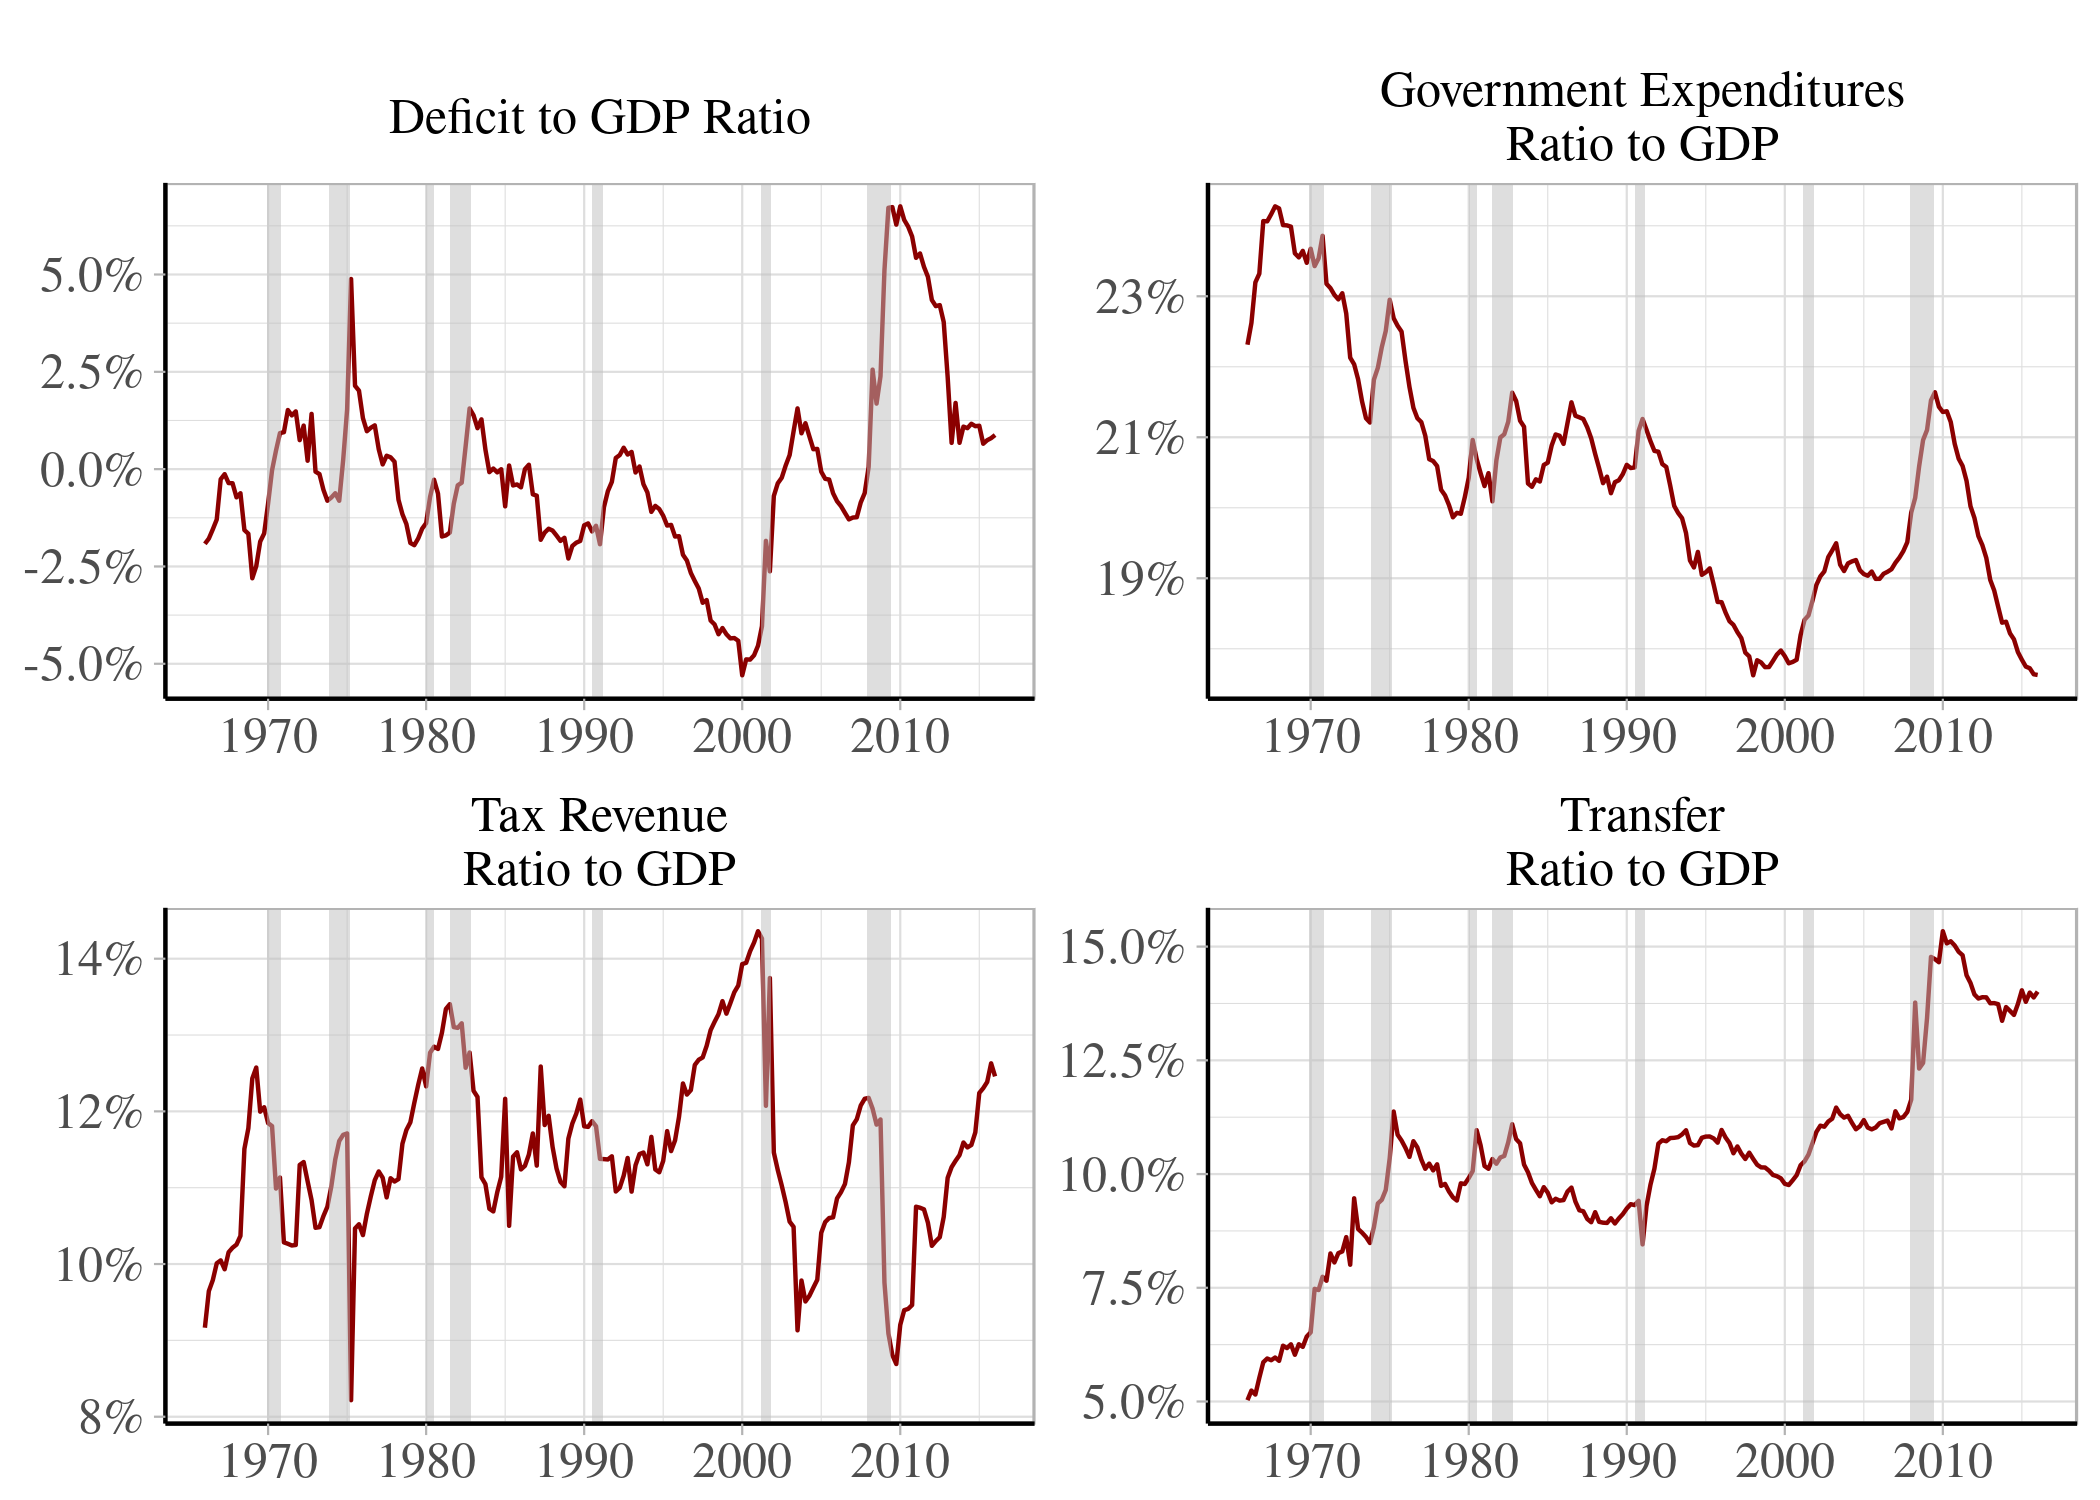
\includegraphics[align=t,width=0.95\textwidth]{./plots/data.png}
\end{frame}

\begin{comment}
\begin{frame}
  \ft{Fiscal Variables}
  \begin{tabular}{cp{1.5in}}
    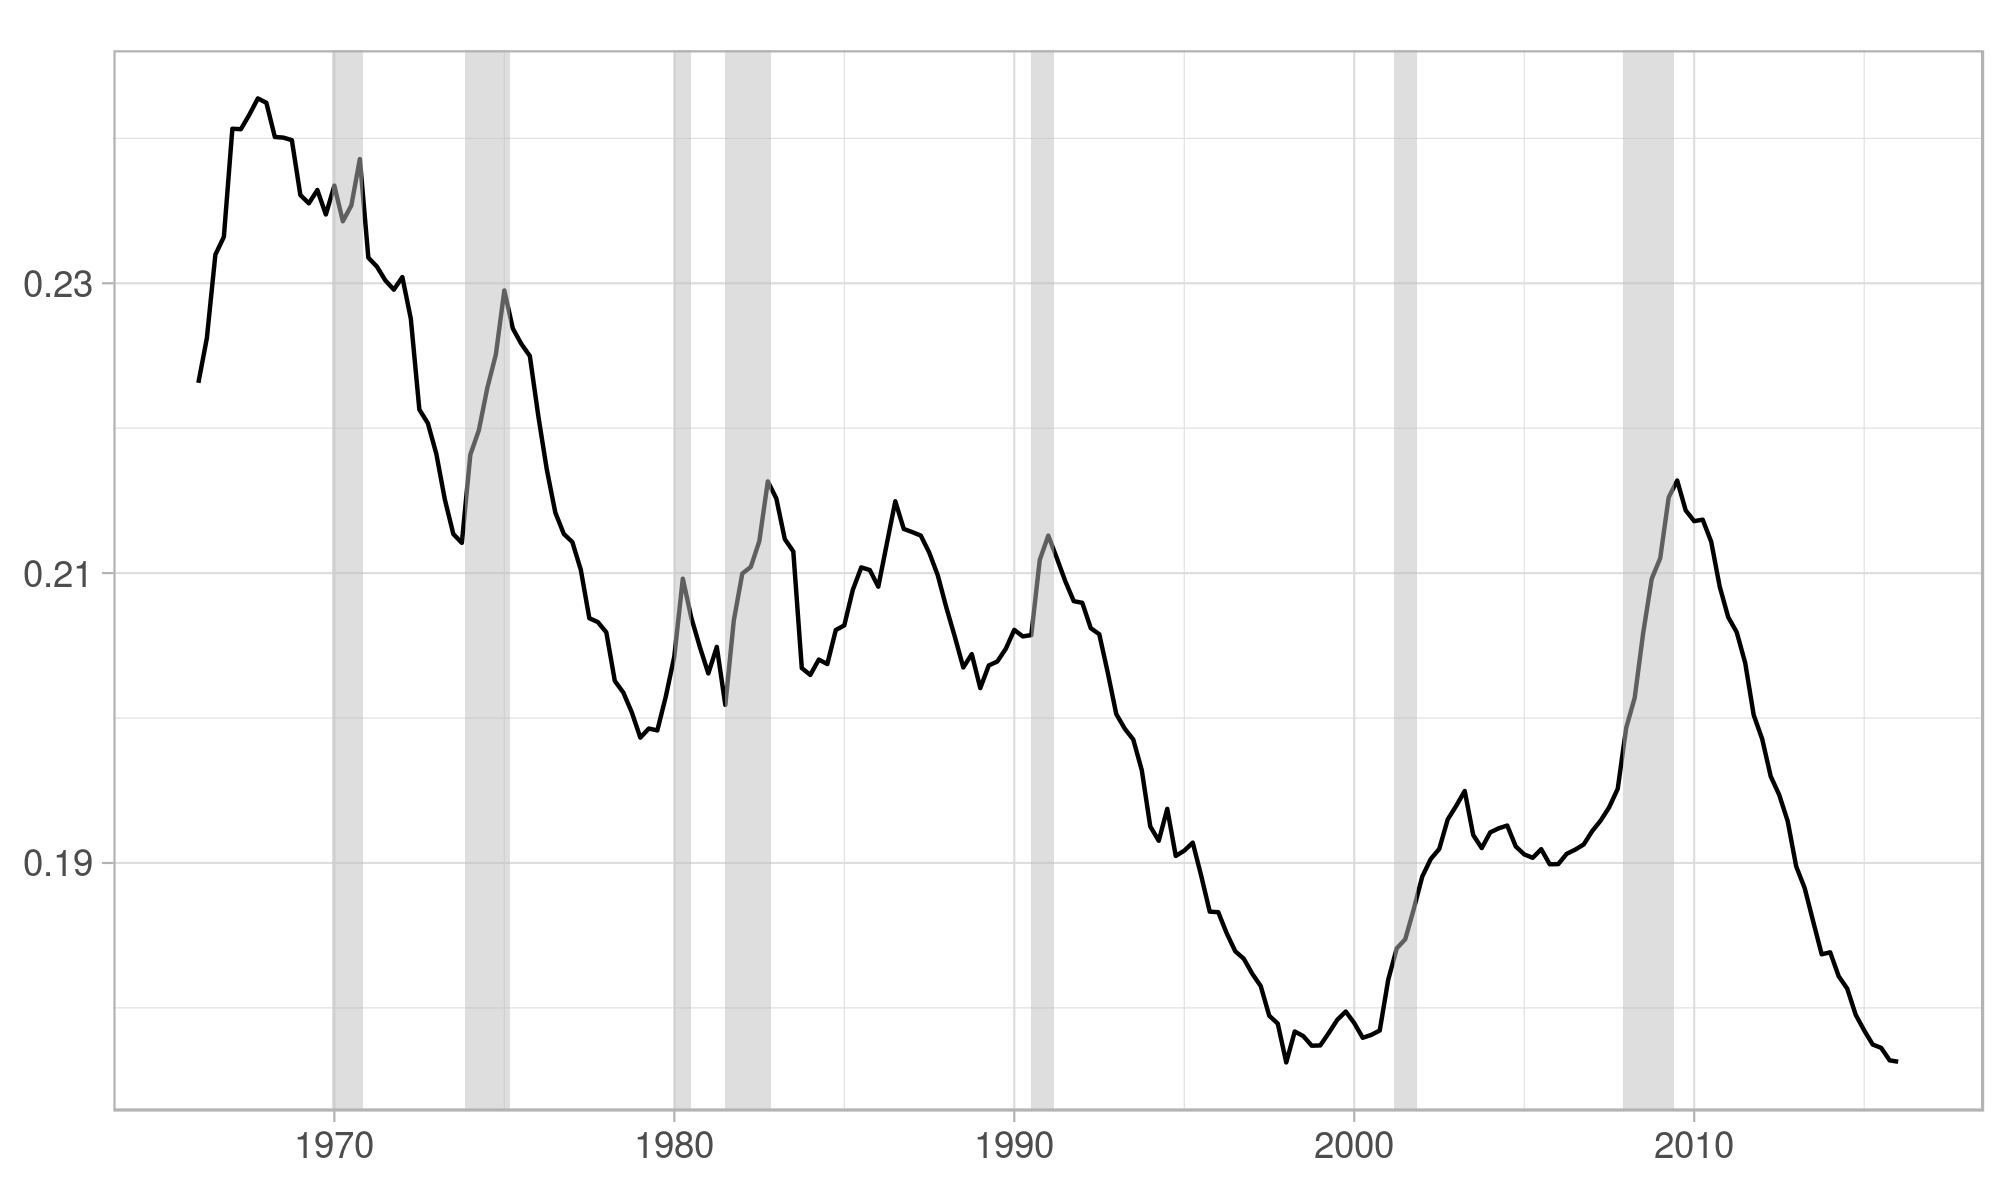
\includegraphics[align=t,height=0.41\textheight]{./gov.png} & \vspace*{2pc}Government Spending / GDP Ratio \\
    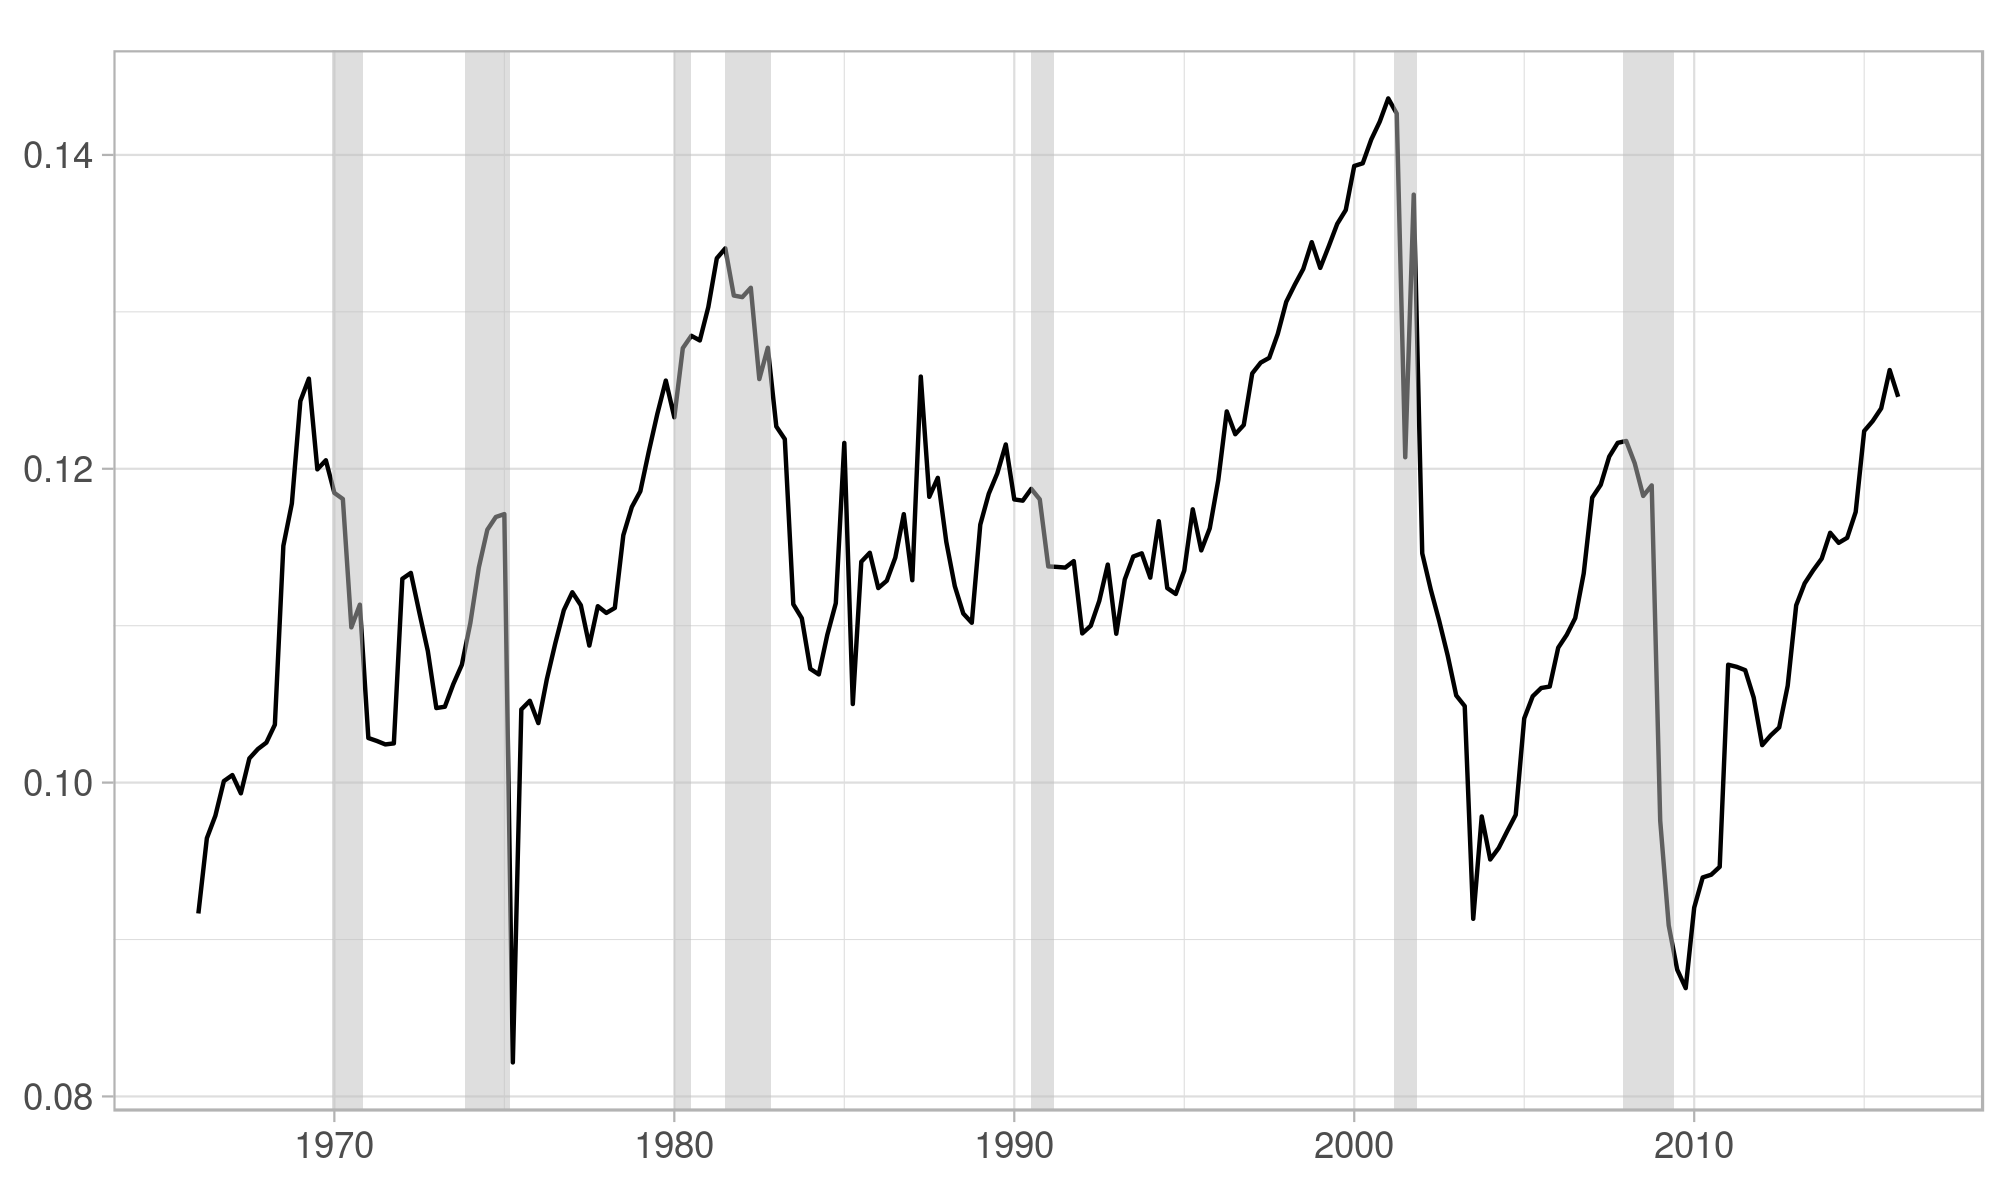
\includegraphics[align=t,height=0.41\textheight]{./tax.png} & \vspace*{2pc}Federal Tax Revenue / GDP Ratio \\
  \end{tabular}
\end{frame}

\begin{frame}
  \ft{Fiscal Variables}
  \begin{tabular}{cp{1.5in}}
    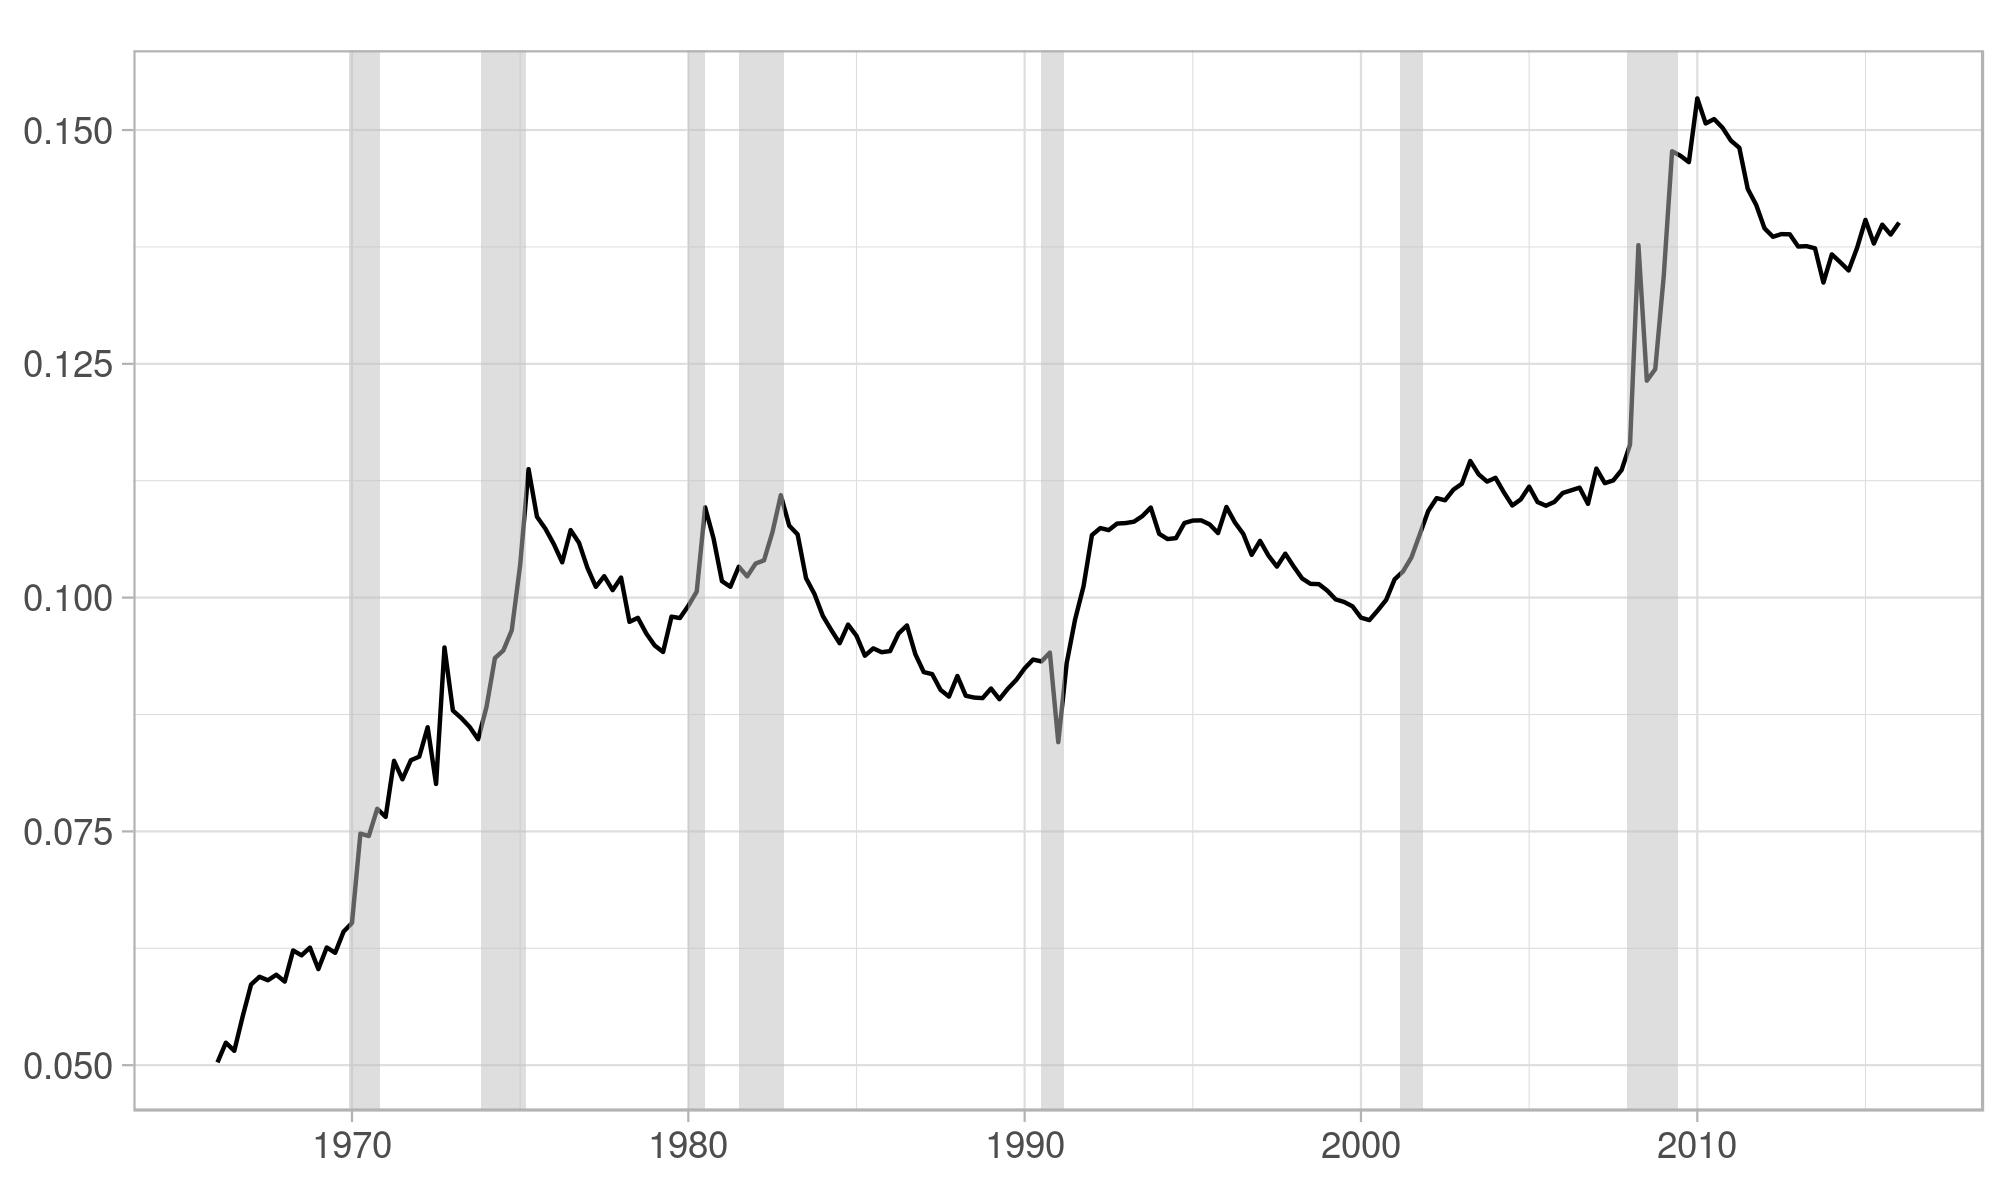
\includegraphics[align=t,height=0.41\textheight]{./transfers.png} & \vspace*{2pc}Transfers / GDP Ratio \\
    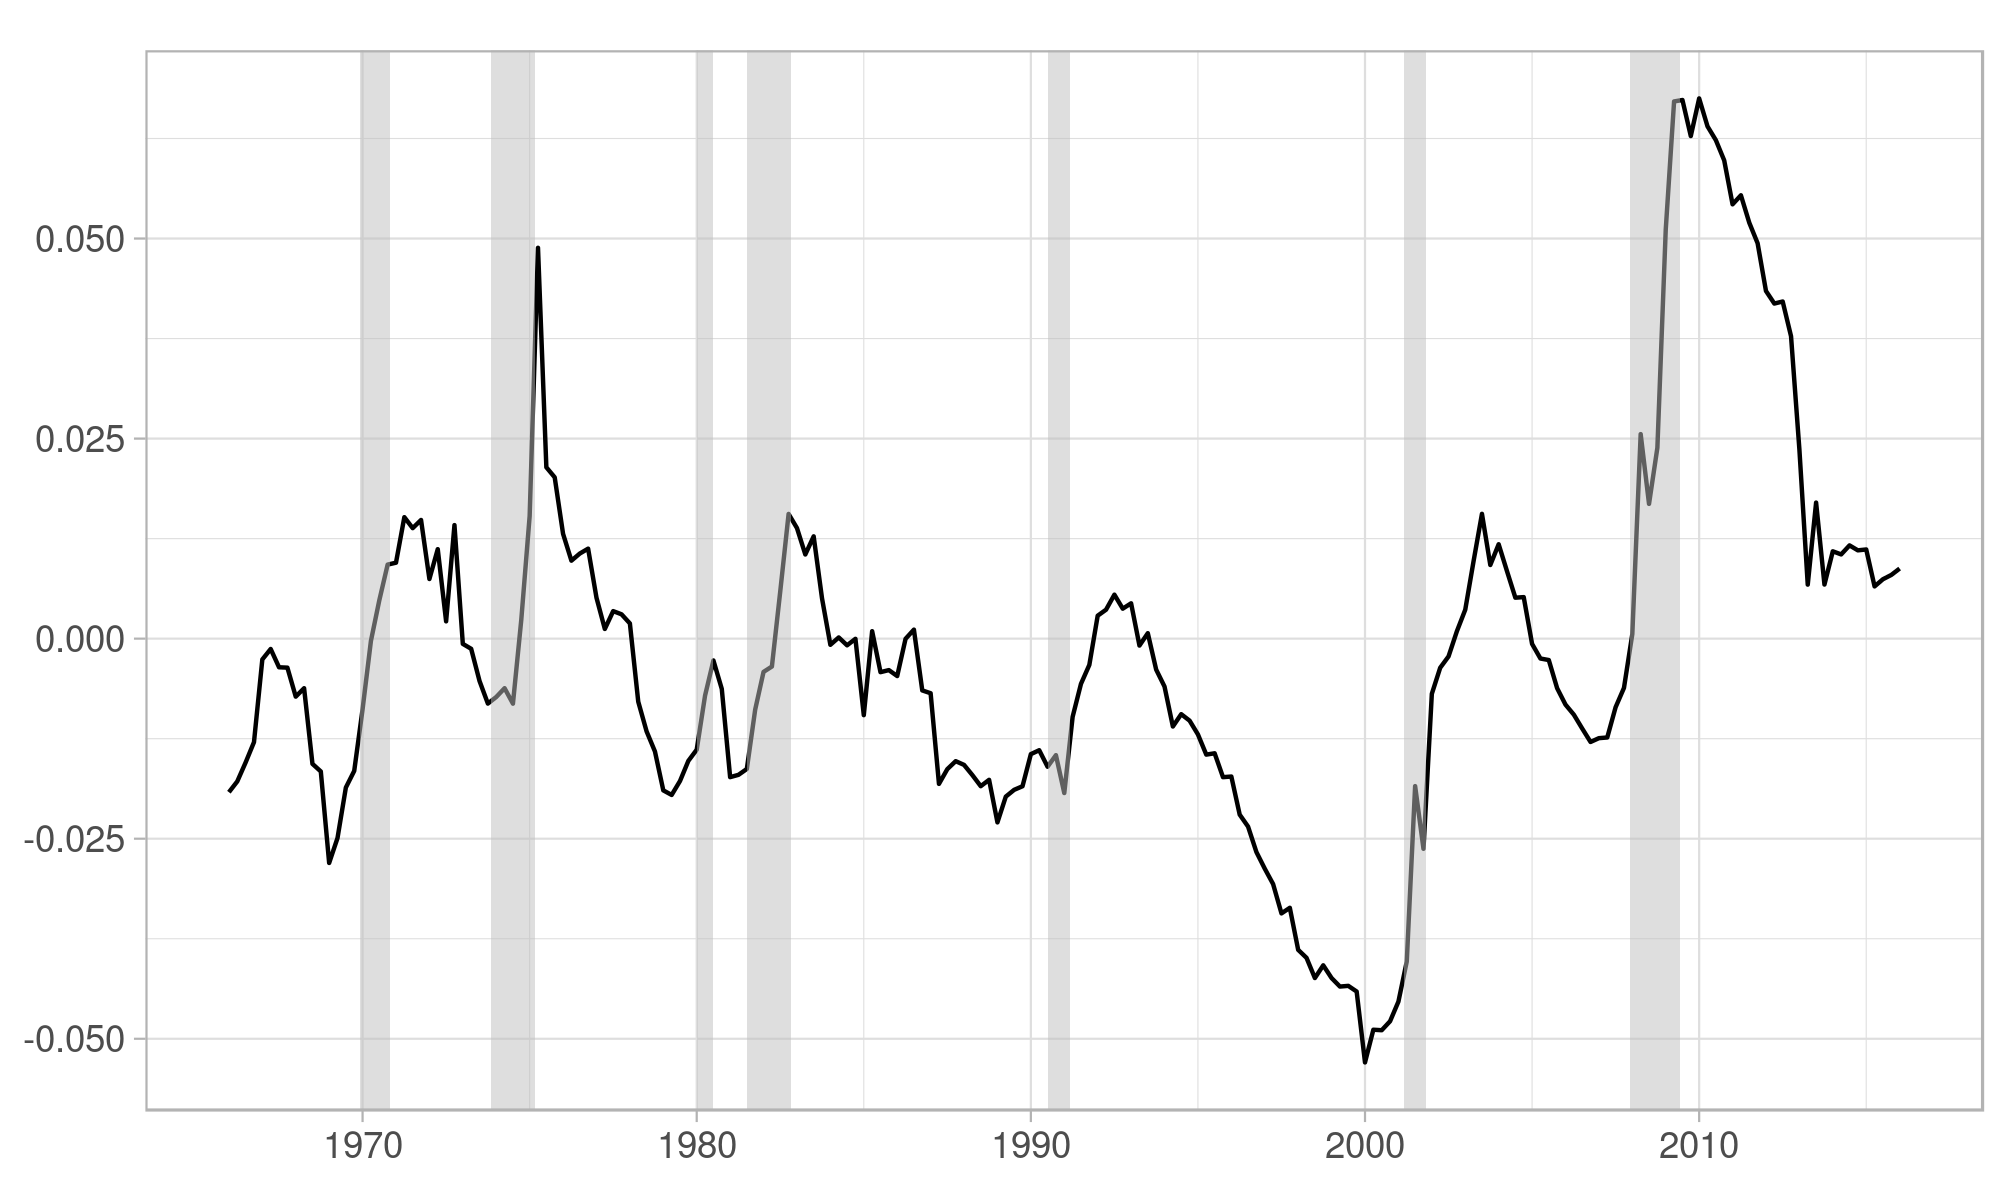
\includegraphics[align=t,height=0.41\textheight]{./deficit.png} & \vspace*{2pc}Deficit / GDP Ratio \\
  \end{tabular}
\end{frame}

\begin{frame}
  \ft{Fiscal Variables}
  \begin{tabular}{cp{1.5in}}
    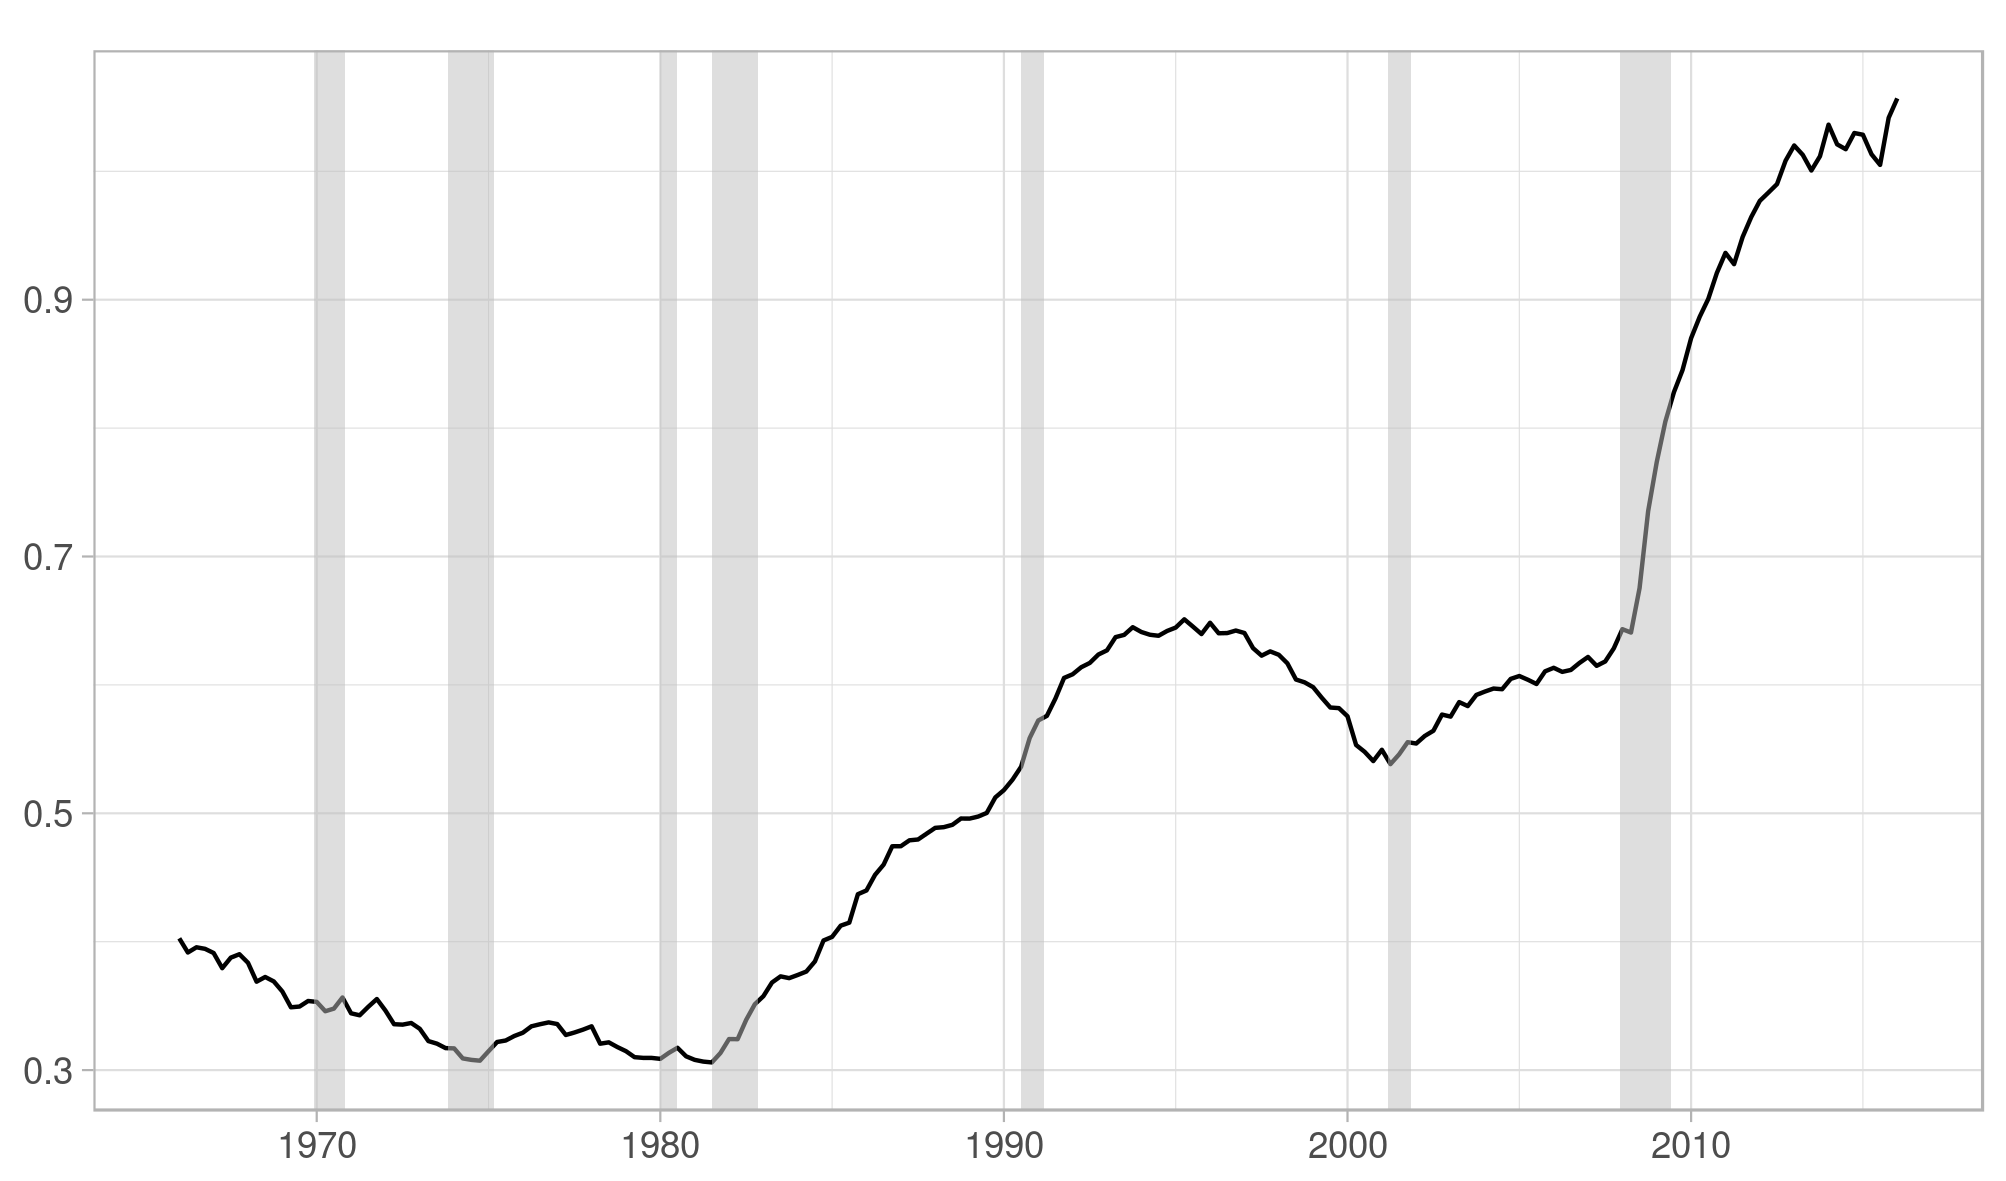
\includegraphics[align=t,height=0.41\textheight]{./debt.png} & \vspace*{2pc}Debt / GDP Ratio \\
  \end{tabular}
\end{frame}
\end{comment}

\begin{frame}
  \ft{Fiscal dynamics matter}
  \uncover<+-> {
    \begin{block}{Debt target and tax response matter}
      \bi
      \item Expected smaller debt/GDP target and/or expected larger response of taxes to debt,\newline
        $\rightarrow$ Higher expected income taxes\newline
        $\rightarrow$ lower consumption, investment, real GDP.
      \item Richter and Throckmorton (EER, 2015):
        \bi
        \item Unknown debt targets amplify impact of tax shocks
        \item Uncertain long-run debt targets reduced impact of ARRA, extensions to Bush tax cut
        \ei
    \end{itemize}
  \end{block}
  } % end uncover

  \uncover<+-> {
  \begin{block}{Fiscal composition matters}
    Leeper, Plante, and Traum (JoE, 2010)
    \begin{itemize}
    \item Rich set of fiscal variables responding to debt fits data best
    \item Magnitude of fiscal shocks depend on composition
    \item Fiscal multipliers can have unexpected signs, depending on composition
    \end{itemize}
  \end{block}
  } % end uncover
\end{frame}

\begin{comment}
\begin{frame}
  \ft{Related fiscal policy literature}
    \uncover<+->{
    \begin{block}{Fiscal policy switching}
      \begin{itemize}
      \item Favero and Montecelli (2005): Deficit feedback rule with \textit{Markov~switching}
        \begin{itemize}
        \item Switching explains data better
        \item Deficits switch between \textit{active} and \textit{passive} regimes
        \end{itemize}
      \item Ko and Morita (2013): Switching in government expenditures and taxes in Japan    
      \end{itemize}
    \end{block}
    }

    \uncover<+->{
    \begin{block}{Switching and Monetary/Fiscal Interactions}
      \begin{itemize}
      \item Eg: Chung, Davig, Leeper (2007), Davig and Leeper (2011)
      \item Evidence for switching between active/passive fiscal and monetary policies
      \item Implications for fiscal multipliers and stabilizing impact of monetary policy
      \end{itemize}
    \end{block}
    }
\end{frame}
\end{comment}

\begin{frame}
  \ft{Fiscal Policy: Government Expenditures}
  \small{
  \uncover<+->{\begin{block}{Gradual movement toward target} 
  \bdm G_t = \rho_g \left(\frac{Y_{t-1}}{Y_{t-2}}\right) G_{t-1} + \left(1-\rho_g\right) G_t^*, \edm
  \vspace*{-1pc}\begin{itemize}\setlength{\itemsep}{0pc}
    \item $\rho_g \in (0,1)$ persistence parameter
    \item $G_t$: Actual nominal government expenditures
    \item $G_t^*$: Target level for government expenditures
    \item $Y_t$: Nominal GDP, so $Y_{t-1}/Y_{t-2}$, is lagged gross NGDP growth.
  \end{itemize}
  \end{block}}
 
  \uncover<+->{\begin{block}{Divide by nominal GDP ($Y_t$)}
  \bdm g_t = \rho_g \left( \frac{y_{t-1}}{y_t} \right) g_{t-1} + \left(1-\rho_g\right) g_t^* \edm
  \vspace*{-0.2pc}\begin{itemize}\setlength{\itemsep}{0pc}
    \item $g_t \equiv G_t/Y_t$, $g_t^* \equiv G_t^*/Y_t$: Actual / Target government expenditures to GDP ratio
    \item $y_t \equiv Y_t/Y_{t-1}$: Gross growth rate of nominal GDP
  \end{itemize}
  \end{block}}
  }
\end{frame}

\begin{frame}
  \ft{Fiscal Policy: Government Expenditures Target}
  \small{
  \uncover<+->{
  \begin{block}{Target Policy Behavior}
    \begin{itemize}\setlength{\itemsep}{0pc}
    \item Use government expenditures to stabilize business cycle\\
      $\rightarrow$ \textbf{Decrease gov exp} in response to output gap 
    \item \textbf{Decrease government expenditures} in response to rising debt
    \end{itemize}
  \end{block}
  }
  \uncover<+->{
  \begin{block}{Structure}
    \bdm g_t^* = \bar{g}(s_t) + \psi_g(s_t) x_t + \gamma_g(s_t) \left[ b_{t-1} - \bar{b}(s_t) \right] + u_{g,t}, \edm
    \vspace*{-1.5pc}\begin{itemize}\setlength{\itemsep}{0pc}
    \item $s_t \in \{1,..,M\}$: Fiscal regime... more later
    \item $\bar{g}(s_t)$: Long-run government expenditures / GDP goal
    \item $b_{t-1}$: Lagged government debt / GDP ratio
    \item $\bar{b}(s_t)$ Long-run goal debt / GDP ratio
    \item $\psi_g(s_t) < 0$: Response to increase in output gap
    \item $\gamma_g(s_t)<0$: Response to increase in government debt
    \item $u_{g,t}$: Shock to government expenditures
    \end{itemize}
  \end{block}
  }
  }
\end{frame}

\begin{frame}
  \ft{Fiscal Policy: Tax Revenue}
  \small{
  \uncover<+->{
    \begin{block}{Movement Toward Target}
      \bdm \tau_t = \rho_\tau \left( \frac{y_{t-1}}{y_t} \right) \tau_{t-1} + \left(1-\rho_\tau\right) \tau_t^* \edm
      \vspace*{-1pc}\bi\setlength{\itemsep}{0pc}
      \item $\tau$, $\tau^*$: Tax revenue / GDP, short-run target
      \ei
    \end{block}
  }

  \uncover<+->{
  \begin{block}{Target Policy Behavior}
    \begin{itemize}\setlength{\itemsep}{0pc}
    \item Use taxes to stabilize business cycle\\
      $\rightarrow$ \textbf{Increase taxes} in response to output gap 
    \item \textbf{Increase taxes} in response to rising debt
    \end{itemize}
  \end{block}
  }
  
  \uncover<+->{
    \begin{block}{Target Tax Policy}
      \bdm \tau_t^* = \bar{\tau}(s_t) + \psi_\tau(s_t) x_t + \gamma_\tau(s_t) \left[ b_{t-1} - \bar{b}(s_t) \right] + u_{\tau,t} \edm
      \vspace*{-1.4pc}\bi\setlength{\itemsep}{0pc}
      \item $\psi_\tau(s_t)>0$: Response to increase in output gap
      \item $\gamma_\tau(s_t)>0$: Response to increase in government debt
      \item $u_{\tau,t}$: Shock to tax policy
      \ei
    \end{block}
  }}
\end{frame}


\begin{frame}
  \ft{Fiscal Policy: Net Transfers}
  \small{
  \uncover<+->{
    \begin{block}{Movement Toward Target}
      \bdm n_t = \rho_n \left( \frac{y_{t-1}}{y_t} \right) n_{t-1} + \left(1-\rho_n\right) n_t^* \edm
      \vspace*{-1pc}\bi\setlength{\itemsep}{0pc}
      \item $n$, $n^*$: Net transfers / GDP, short-run target
      \ei
    \end{block}
  }

  \uncover<+->{
  \begin{block}{Target Policy Behavior}
    \begin{itemize}\setlength{\itemsep}{0pc}
    \item Use transfers to stabilize business cycle\\
      $\rightarrow$ \textbf{Decrease transfers} in response to output gap 
    \item \textbf{Decrease transfers} in response to rising debt
    \end{itemize}
  \end{block}
  }
  
  \uncover<+->{
    \begin{block}{Target Transfers Policy}
      \bdm n_t^* = \bar{n}(s_t) + \psi_n(s_t) x_t + \gamma_n(s_t) \left[ b_{t-1} - \bar{b}(s_t) \right] + u_{n,t} \edm
      \vspace*{-1.4pc}\bi\setlength{\itemsep}{0pc}
      \item $\psi_n(s_t)<0$: Response to increase in output gap
      \item $\gamma_n(s_t)<0$: Response to increase in government debt
      \item $u_{n,t}$: Shock to transfers policy
      \ei
    \end{block}
  }}
\end{frame}

\begin{frame}
  \ft{Budget Deficit}
  \uncover<+->{
    \begin{block}{Primary Budget Deficit}
      \bdm d_t = \tau_t - g_t - n_t + \tilde{d}_t \edm
      $\tilde{d}_t$: Deficit residual\newline
      \hspace*{1.2pc}(Other expenditure or revenue items I did not include)
    \end{block}
  }
  \uncover<+->{
    \begin{block}{Deficit Residual Behavior}
      Gradual movement toward target:
      \bdm \tilde{d}_t = \rho_d \left( \frac{y_{t-1}}{y_t} \right) \tilde{d}_{t-1} + \left(1-\rho_d\right) d_t^* \edm
      Short-run target:
      \bdm d_t^* =\bar{\tilde{d}}(s_t) + \psi_d(s_t) x_t + \gamma_d(s_t) \left[ b_{t-1} - \bar{b}(s_t) \right] + u_{d,t} \edm
    \end{block}
  }
\end{frame}


\begin{frame}
  \ft{Government Budget Constraint}
  \begin{small}
  \uncover<+->{
  \begin{block}{Intertemporal government budget constraint}
  \bdm B_t = (1 + r_{t-1}) B_{t-1} + D_t - \left( M_t - M_{t-1} \right), \edm
  \begin{tabular}{ll}
    $B_t$: Nominal government debt & $r_{t-1}$: interest rate on past-issued debt \\
    $D_t$: Nominal budget deficit & $M_t - M_{t-1}$: seigniorage
  \end{tabular}
  \end{block}
  }

  \uncover<+->{
  \begin{block}{Empirical government budget constraint}
    Divide both sides by $Y_t$ and allow for measurement error ($v_t$)
    \only<1-2>{\bdm b_t = (1+r_{t-1}) \left(\frac{1}{y_t}\right) b_{t-1} + d_t - m_t + \left(\frac{1}{y_t}\right) m_{t-1} + v_t \edm
      \vspace*{5pc} }
    \only<3->{\bdm b_t = (1+r_{t-1}) \left(\frac{1}{y_t}\right) b_{t-1} + d_t \textcolor{red}{\underbrace{\displaystyle~ -~ m_t + \left(\frac{1}{y_t}\right) m_{t-1} + v_t}_{\mbox{Residual: } \displaystyle u_{b,t}}} \edm
    }
    \only<3>{\vspace*{3.55pc}}
    \only<4->{
    \bdm b_t = (1+r_{t-1}) \left(\frac{1}{y_t}\right) b_{t-1} + d_t + u_{b,t} \edm
    }
  \end{block}
  }
  \end{small}
\end{frame}

\begin{frame}
  \ft{Relationship between deficits and debt}
  \uncover<+->{\begin{block}{Budget constraint}
  \bi
\item Budget constraint describes relationship between long-run targets for...\\
  $~~$(1) Debt / GDP, $\bar{b}(s_t)$, and\\
  $~~$(2) deficits / GDP, $\bar{d}(s_t)$
  \item Evaluate budget constraint at steady state and a constant fiscal regime $s_{t-1}=s_t=s$:
    \bdm \bar{d}(s) = \left( \frac{\bar{y}-\bar{r}-1}{\bar{y}} \right) \bar{b}(s) - \bar{u}_b \edm
    \ei
  \end{block}}

  \uncover<+->{
  \begin{block}{Long-run deficit dependencies}
    \begin{tabular}{ll}
    Debt target & Long-run nominal interest rate \\
    Long-run nominal GDP growth & Long-run seigniorage 
    \end{tabular}
    
    \ \\
    Jointly estimate these long-run targets 
  \end{block}}  
\end{frame}

\begin{frame}
  \ft{Variances}
  
  \uncover<+->{
  \begin{block}{Regime-dependent variances for fiscal shocks}
    \begin{tabular}{ll}
      $\sigma_g^2(s_t)$: Var(shock to gov exp) & $\sigma_n^2(s_t)$: Var(shock to transfers) \\
      $\sigma_\tau(s_t)$: Var(shock to taxes) & $\sigma_d^2(s_t)$: Var(shock to deficits) \end{tabular}
  \end{block}}

  \uncover<+->{
  \begin{block}{Correlations of fiscal shocks}
    \begin{itemize}
    \item Fiscal policy decisions are dependent on one another.
    \item Consider all possible correlations:\\
      \hspace{2pc} $\varrho_{g,\tau}$, $\varrho_{\tau,n}$, $\varrho_{g,n}$, $\varrho_{\tau,d}$, $\varrho_{g,d}$, $\varrho_{n,d}$
    \end{itemize}
  \end{block}
  }
\end{frame}

\begin{frame}
  \ft{Three Sources for Regime Switching}
  \begin{footnotesize}
  \uncover<+->{\begin{block}{Long-run Debt Target Regimes}
    \begin{enumerate}[{Regime} A:]
      \setcounter{enumi}{11}
      \item \textit{Low} long-run target for debt/GDP (low value for  $\bar{b}(s_t)$)
      \setcounter{enumi}{7}
      \item \textit{High} long-run target for debt/GDP (high value for  $\bar{b}(s_t)$)
    \end{enumerate}
  \end{block}}

  \uncover<+->{
    \begin{block}{Fiscal Financing}
      \bi
      \item Targets for fiscal components: $\bar{g}(s_t)$, $\bar{\tau}(s_t)$, $\bar{n}(s_t)$, $\bar{d}(s_t)$
      \item Behavior toward output gap and debt: $\psi_f(s_t)$ and $\gamma_f(s_t)$, for $f \in \{g,\tau,n,\tilde{d}\}$
      \ei
        
      \vspace*{-0.5pc}\begin{enumerate}[{Regime} A:]
      \item Fiscal behavior A
      \item Fiscal behavior B
      \end{enumerate}
    \end{block}
  }

  \uncover<+->{
    \begin{block}{Fiscal Volatility}
      Two regimes to determine variances, $\sigma_g^2(s_t)$, $\sigma_\tau^2(s_t)$, $\sigma_n^2(s_t)$, and $\sigma_d^2(s_t)$:
      \begin{enumerate}[{Regime} A:]
        \setcounter{enumi}{18}
        \item \textit{Stable}, relatively smaller variances
        \setcounter{enumi}{21}
        \item \textit{Volatile}, relatively larger variances 
      \end{enumerate}
    \end{block}
  }
  \end{footnotesize}
  
\end{frame}

\begin{frame}
  \ft{Regime Switching Procedure}
  \begin{footnotesize}
  \uncover<+-> {
  \begin{block}{Markov regime switching}
    Regime switches randomly, each source \textbf{independently} of other sources
    \bi
    \item $p_L=P(s_t=L | s_{t-1}=L)$ be prob policy remains in reg L
    \item $p_H=P(s_t=H | s_{t-1}=H)$ be prob policy remains in reg H
    \item $p_A=P(s_t=A | s_{t-1}=A)$ be prob policy remains in reg A
    \item $p_A=P(s_t=B | s_{t-1}=B)$ be prob policy remains in reg B
    \item $p_A=P(s_t=S | s_{t-1}=S)$ be prob policy remains in reg S
    \item $p_A=P(s_t=V | s_{t-1}=V)$ be prob policy remains in reg V
    \ei
  \end{block}}

  \uncover<+->{\begin{block}{Rich Set of Regime-Switching Possibilities} 
      \bi
      \item Changes in priorities for taxes, transfers, spending, \textit{without adjusting long-run targets for debt/GDP}
      \item Changes in debt-targets, \textit{without adjusting purposes and priorities for fiscal components}
      \item Changes in volatility of fiscal outcomes, \textit{without changing goals or purposes}
      \ei
  \end{block}}
  \end{footnotesize}
\end{frame}

\begin{frame}
  \ft{Completing the model}
  \uncover<+->{\begin{block}{Loose ends}
  \bi
  \item Relationship between $\bar{d}(s_t)$ and $\bar{b}(s_t)$ depends on...
    \bi
    \item long-run values for nominal GDP growth ($\bar{y}$)
    \item long-run average interest rate ($\bar{r}$)
    \ei  
  \item Identify effects of output gap on fiscal policy behavior \textit{from effects of fiscal policy actions on output gap}.
  \ei
  \end{block}}

  \uncover<+->{\begin{block}{Next steps}
    \bi
    \item Specify monetary policy
    \item Specify inter-dependent behavior of macro variables:\newline GDP growth, output gap, and inflation
    \ei
  \end{block}}
\end{frame}

\begin{frame}
  \ft{Monetary Policy}
  \uncover<+->{\begin{block}{Taylor-like (1993) rule}
  \bdm r_t = (1-\rho_r) \bar{r} + \rho_r r_{t-1} + (1-\rho_r) \left[\phi_x x_t + \phi_\pi \left(\pi_t - \bar{\pi}\right) \right] + u_{r,t}, \edm
  \begin{tabular}{ll}
    $\bar{r}$: long-run nominal interest rate & $\pi_t$: inflation rate \\
    $\rho_r$: Monetary policy persistence & $\bar{\pi}$: target inflation rate \\
    $\phi_x > 0$: Response to output gap & $x_t$: output gap \\
    $\phi_\pi >0$: Response to inflation & $u_{r,t}$: shock to monetary policy \\
  \end{tabular}
  \end{block}}

  \uncover<+->{\begin{block}{Policy shock}
      \bdm u_{r,t} = \alpha_r u_{r,t-1} + e_{r,t}, ~~ e_{r,t} \sim \mathcal{N}\left(0, \sigma_r^2\right) \edm
  \end{block}}
\end{frame}

\begin{frame}
  \ft{Output and Inflation Dynamics}
  \uncover<+->{\begin{block}{Dependent variables}
  Augmented vector autoregression for...
  \be
  \item nominal GDP growth, $y_t$,
  \item output gap, $x_t$, 
  \item inflation, $\pi_t$
  \ee
  \end{block}}

  \uncover<+->{\begin{block}{Explanatory variables}
    \bi
    \item One lag of all dependent variables: $y_{t-1}$, $x_{t-1}$, $\pi_{t-1}$
    \item Fiscal policy variables: $g_t$, $\tau_t$, $n_t$
    \item Monetary policy: $r_t$
      \ei
  \end{block}}

  \uncover<+->{\begin{block}{Estimation Outcomes}
    \bi
    \item Long-run values for $\bar{y}$ and $\bar{r}$
    \item Predictive model for impact of fiscal policy on macro outcomes, $y_t$, $x_t$, $\pi_t$, $r_t$
    \ei
  \end{block}}
      
\end{frame}

\begin{frame}
  \ft{Data}
  \begin{footnotesize}

  \uncover<+->{\begin{block}{Fiscal policy variables}
  \be
  \item Nominal government expenditures: NIPA Table 1.1.5, Line 22
  \item Tax revenue: NIPA Table 3.2, Line 3
  \item Net transfers: Federal current transfer pmts - receipts
    \bi \item NIPA Table 3.2, (Line 25 - Line 18) \ei
  \item Primary budget deficit:
    \bi \item (-) net federal government saving - federal interest payments
    \item NIPA Table 3.2, Line 36 - Line 32 \ei
  \item Government debt: Federal debt held by the public (U.S. Dept of Treasury)
  \ee
  \end{block}}

  \uncover<+->{\begin{block}{Remaining variables}
    \be
    \setcounter{enumi}{5}
    \item Nominal GDP: NIPA Table 1.1.5, Line 1
    \item Output gap: Difference between NGDP and potential GDP 
    \item Inflation: Growth GDP implicit price deflator (NIPA Table 1.1.9, Line 1)
    \item Interest rate: Federal funds rate
      \ee
  \end{block}}
  \end{footnotesize}
\end{frame}

\begin{comment}
\begin{frame}
  \ft{State / Space System}
  State equation with regime switching:
  \bdm \xi_t = h^*(s_t) + F^*(s_t) \xi_{t-1} + M^* e_t, ~~e_t \sim \mathcal{N}\left(0, Q(s_t) \right) \edm

  \begin{center}
  \begin{footnotesize}
  \begin{tabular}{cc}
    State Vector: $\xi_t$ & Stochastic vector: $e_t$ \\ \hline
    $g_t$ and $g_t^*$ & $e_{g,t}$ \\
    $\tau_t$ and $\tau_t^*$ &  $e_{\tau,t}$ \\
    $n_t$ and $n_t^*$ &  $e_{n,t}$ \\
    $d_t$ &  $e_{d,t}$ \\
    $b_t$ and $b_t^*$ &  $e_{b,t}$ \\
    $y_t$, & $e_{y,t}$ \\
    $x_t$, & $e_{x,t}$ \\
    $pi_t$, & $e_{\pi,t}$ \\
    $r_t$ &  $e_{r,t}$ \\
    AR(1) shocks & \\ \hline
  \end{tabular}
  \end{footnotesize}
  \end{center}

  Observation equation: Indicator matrix picking off observable values in state vector 
\end{frame}
\end{comment}

\begin{frame}
  \ft{Estimation}
  \small{
  \uncover<+->{\begin{block}{Kim filter}
  \bi
  \item Kim and Nelson (1999): Extend Kalman filter with regime-dependent coefficients and variances
  \item Approximates probability in each regime over sample period, \textit{given parameters, including switching probabilities}.
  \ei
  \end{block}}
  
  \uncover<+->{
  \begin{block}{Bayesian Estimation}
  \bi
  \item Metropolis-Hastings Markov-Chain Monte Carlo
  \item Impose $(0,1)$ priors for a number of parameters (persistence, fiscal components ratio to GDP, et al.)
  \item Impose sign restrictions on priors for several parameters, eg:
    \bi
    \item Fiscal policy responses to output gap and debt/GDP
    \item Monetary policy responses to output gap
    \item Long-run average NGDP growth, inflation, interest rate
    \ei
  \ei
  \end{block}
  }}
\end{frame}

\begin{frame}
  \begin{small}
  \ft{Sign Restrictions on Impulse Response Functions}
  \uncover<+->{
  \begin{block}{Endogoneity problem: two-way causation}
    \bi
    \item \textit{Ceteris paribus}, an increase in output gap leads to higher taxes (captured by parameter $\psi_{\tau}(s_t)$ in fiscal policy equation)
    \item \textit{Ceteris paribus}, an increase in taxes leads lower aggregate demand and therefore a lower output gap (captured by coef in augmented VAR for $x_t$)
    \ei
  \end{block}}

  \uncover<+->{
  \begin{block}{Sign restrictions}
    \bi\setlength{\itemsep}{0pt}
    \item Faust (1998), Canova and De Nicolo (2002), and Uhlig (2005)
    \item MCMC parameter draw used to compute \textit{impulse response functions}.
    \item Impulse response function examples:
      \vspace*{-0.2pc}\bi\setlength{\itemsep}{0pt}
      \item Impulse = single shock to output gap
      \item Response = time path of response to tax revenue
      \item Response = time path of response to output gap
      \ei
    \item Require some responses be non-negative or non-positive    
    \ei
  \end{block}}
  \end{small}
\end{frame}

\begin{frame}
  \ft{Example Sign Restrictions}
  \uncover<+->{
  \begin{block}{Impulse: Shock to output gap}
      \bi
      \item Responses = resulting time paths for output gap, tax revenue
      \item Output gap response should be positive
      \item Tax revenue response should be positive
        \ei
  \end{block}}
  \uncover<+->{
  \begin{block}{Impulse: Shock to tax ratio}
      \bi
      \item Responses = resulting time paths for output gap, tax revenue
      \item Output gap response should be negative
      \item Tax revenue response should be positive
        \ei
  \end{block}}

  \uncover<+->{
    \begin{block}{Time frame}
      Restrict cumulative response over \textit{2 quarters}, including shock period.
    \end{block}
  }
\end{frame}

\begin{frame}
  \ft{Fiscal Policy Sign Restrictions}
  \uncover<+->{
  \begin{block}{Fiscal policy sign restrictions}
  \begin{footnotesize}
  \begin{tabular}{lccccc}
    & \multicolumn{5}{c}{\textbf{Impulse Variable}} \\ 
    \textbf{Response} & Gov Exp & Taxes & Transfers & Deficit & Output gap\\ \hline
    Output gap & \textcolor{blue}{positive} & \textcolor{red}{negative} & \textcolor{blue}{positive} & \textcolor{blue}{positive} & \textcolor{blue}{positive} \\
    Output growth & \textcolor{blue}{positive} & \textcolor{red}{negative} & \textcolor{blue}{positive} & \textcolor{blue}{positive} & \textcolor{blue}{positive}\\
    Gov exp & \textcolor{blue}{positive} & (none) & (none) & (none) & \textcolor{red}{negative} \\
    Taxes & (none) & \textcolor{blue}{positive} & (none) & (none) & \textcolor{blue}{positive} \\
    Transfers & (none) & (none) & \textcolor{blue}{positive} & (none) & \textcolor{red}{negative} \\
    Deficits & (none) & (none) & (none) & \textcolor{blue}{positive}  & \textcolor{red}{negative} \\ \hline
  \end{tabular}
  \end{footnotesize}
  \end{block}}

  \uncover<+->{
  \begin{block}{Monetary policy sign restrictions}
  \begin{center}
  \begin{footnotesize}
  \begin{tabular}{lccc}
    & \multicolumn{3}{c}{\textbf{Impulse Variable}} \\ 
    \textbf{Response} & Interest rate & Output gap & Inflation \\ \hline
    Output gap & \textcolor{red}{negative} & \textcolor{blue}{positive} & (none)  \\
    Output growth & \textcolor{red}{negative} & \textcolor{blue}{positive} & (none)  \\
    Inflation & \textcolor{red}{negative} & \textcolor{blue}{positive} & (none)  \\
    Interest rate & \textcolor{blue}{positive} & \textcolor{blue}{positive} & \textcolor{blue}{positive} \\ \hline
  \end{tabular}
  \end{footnotesize}
  \end{center}
  \end{block}}
\end{frame}

\begin{frame}
  \ft{Results: Government Expenditures Behavior}
  \small{
    \uncover<+->{\begin{block}{Posterior Parameter Distributions Under Regimes A \& B}
      \setlength{\tabcolsep}{2pt}
      \begin{tabular}{clcccc}
        & & \multicolumn{2}{c}{Fiscal Regime A} & \multicolumn{2}{c}{Fiscal Regime B} \\ 
        Param. & Description & Median & 90\% Bounds & Median & 90\% Bounds \\ \hline
        \hl{2}{$\bar{g}$} & \hl{2}{Long-run gov target} & \hl{2}{0.19} & \hl{2}{(0.18, 0.20)} & \hl{2}{0.31} & \hl{2}{(0.29, 0.32)} \\ [0.2pc]
        \hl{3}{$\psi_{g}$} & \hl{3}{Resp to output gap} & \hl{3}{-0.32} & \hl{3}{(-0.38, -0.28)} & \hl{3}{-0.43} & \hl{3}{(-0.45, -0.39)} \\ [0.2pc]
        \hl{4}{$\gamma_{g}$} & \hl{4}{Resp to debt} & \hl{4}{-0.55} & \hl{4}{(-0.61, -0.49)} & \hl{4}{-0.44} & \hl{4}{(-0.50, -0.40)} \\ \hline
      \end{tabular}
    \end{block}}

    \uncover<+->{\begin{block}{Description}
      \bi
      \item<2> \hl{2}{Fiscal Regime A has \textbf{lower long-run} government expenditures}
      \item<3> \hl{3}{Fiscal regime A has government expenditures \textbf{less responsive to output gap}}
      \item<4> \hl{4}{Fiscal regime A has government expenditures \textbf{more responsive to debt}}
      \ei
    \end{block}
    }
  }
\end{frame}

\begin{frame}
  \ft{Results: Tax Behavior}
  \small{
    \uncover<+->{\begin{block}{Posterior Parameter Distributions Under Regimes A \& B}
      \setlength{\tabcolsep}{2pt}
      \begin{tabular}{clcccc}
        & & \multicolumn{2}{c}{Fiscal Regime A} & \multicolumn{2}{c}{Fiscal Regime B} \\ 
        Param. & Description & Median & 90\% Bounds & Median & 90\% Bounds \\ \hline
        \hl{2}{$\bar{\tau}$} & \hl{2}{Long-run tax target} & \hl{2}{0.14} & \hl{2}{(0.13, 0.14)} & \hl{2}{0.28} & \hl{2}{(0.25, 0.29)} \\ [0.2pc]
        \hl{3}{$\psi_{\tau}$} & \hl{3}{Resp to output gap} & \hl{3}{0.69} & \hl{3}{(0.68, 0.72)} & \hl{3}{0.47} & \hl{3}{(0.44, 0.55)} \\ [0.2pc]
        \hl{4}{$\gamma_{\tau}$} & \hl{4}{Resp to debt} & \hl{4}{0.25} & \hl{4}{(0.23, 0.29)} & \hl{4}{0.34} & \hl{4}{(0.26, 0.44)} \\ \hline
      \end{tabular}
    \end{block}}

    \uncover<+->{\begin{block}{Description}
      \bi
      \item<2> \hl{2}{Fiscal Regime A has \textbf{lower long-run} tax target}
      \item<3> \hl{3}{Fiscal regime A has taxes \textbf{more responsive to output gap}}
      \item<4> \hl{4}{Fiscal regime A has taxes \textbf{less responsive to debt}}
      \ei
    \end{block}
    }
  }
\end{frame}


\begin{frame}
  \ft{Results: Transfers Behavior}
  \small{
    \uncover<+->{\begin{block}{Posterior Parameter Distributions Under Regimes A \& B}
      \setlength{\tabcolsep}{2pt}
      \begin{tabular}{clcccc}
        & & \multicolumn{2}{c}{Fiscal Regime A} & \multicolumn{2}{c}{Fiscal Regime B} \\ 
        Param. & Description & Median & 90\% Bounds & Median & 90\% Bounds \\ \hline
        \hl{2}{$\bar{n}$} & \hl{2}{Long-run transfers} & \hl{2}{0.11} & \hl{2}{(0.10, 0.13)} & \hl{2}{0.18} & \hl{2}{(0.17, 0.20)} \\ [0.2pc]
        \hl{3}{$\psi_{n}$} & \hl{3}{Resp to output gap} & \hl{3}{-0.46} & \hl{3}{(-0.49, -0.41)} & \hl{3}{-0.50} & \hl{3}{(-0.54, -0.43)} \\ [0.2pc]
        \hl{4}{$\gamma_{n}$} & \hl{4}{Resp to debt} & \hl{4}{-0.33} & \hl{4}{(-0.37, -0.26)} & \hl{4}{-0.51} & \hl{4}{(-0.55, -0.47)} \\ \hline
      \end{tabular}
    \end{block}}

    \uncover<+->{\begin{block}{Description}
      \bi
      \item<2> \hl{2}{Fiscal Regime A has \textbf{lower long-run} transfers}
      \item<3> \hl{3}{Regimes are \textbf{not different on responsiveness to output gap}}
      \item<4> \hl{4}{Fiscal regime A has transfers \textbf{less responsive to debt}}
      \ei
    \end{block}
    }
  }
\end{frame}



\begin{frame}
  \ft{Results: Debt Regimes}
  \small{
    \uncover<+->{\begin{block}{Posterior Parameter Distributions Under Low \& High Debt Regimes}
      \setlength{\tabcolsep}{2pt}
      \begin{tabular}{clcccc}
        & & \multicolumn{2}{c}{Low Debt Regime} & \multicolumn{2}{c}{High Debt Regime} \\ 
        Param. & Description & Median & 90\% Bounds & Median & 90\% Bounds \\ \hline
        $\bar{b}$ & Debt/GDP target & 0.37 & (0.34, 0.39) & 0.60 & (0.55, 0.64) \\ \hline
      \end{tabular}
    \end{block}}

    \uncover<.->{\begin{block}{Debt Regimes}
      Low debt regime $\approx$ 37\% of GDP\\
      High debt regime $\approx$ 60\% of GDP
    \end{block}
    }
  }
\end{frame}

\begin{frame}
  \ft{Results: Volatility Regimes}
  \small{
    \uncover<+->{\begin{block}{Posterior Parameter Distributions Under Stable and Volatile Regimes}
       \setlength{\tabcolsep}{4pt}
       \begin{tabular}{clcccc}
        & & \multicolumn{2}{c}{Stable Regime} & \multicolumn{2}{c}{Volatile Regime} \\ 
        Param. & Description & Median & 90\% Bounds & Median & 90\% Bounds \\ \hline
        $\sigma_{g}$ & Gov stdev & 0.10 & (0.09, 0.11) & 0.19 & (0.17, 0.22) \\ 
        $\sigma_{\tau}$ & Tax stdev & 0.10 & (0.10, 0.11) & 0.29 & (0.28, 0.30) \\ 
        $\sigma_{n}$ & Transfers stdev & 0.06 & (0.06, 0.08) & 0.22 & (0.19, 0.26) \\ 
        $\sigma_{d}$ & Deficit stdev & 0.08 & (0.08, 0.10) & 0.20 & (0.19, 0.22) \\ \hline
      \end{tabular}
    \end{block}}
  }
  \ \\
  \textcolor{BrickRed}{All standard deviations are larger in volatile regime,\\\textbf{most more than double}.}
\end{frame}

\begin{frame}
  \ft{Timing of Fiscal Regimes}
  \begin{center}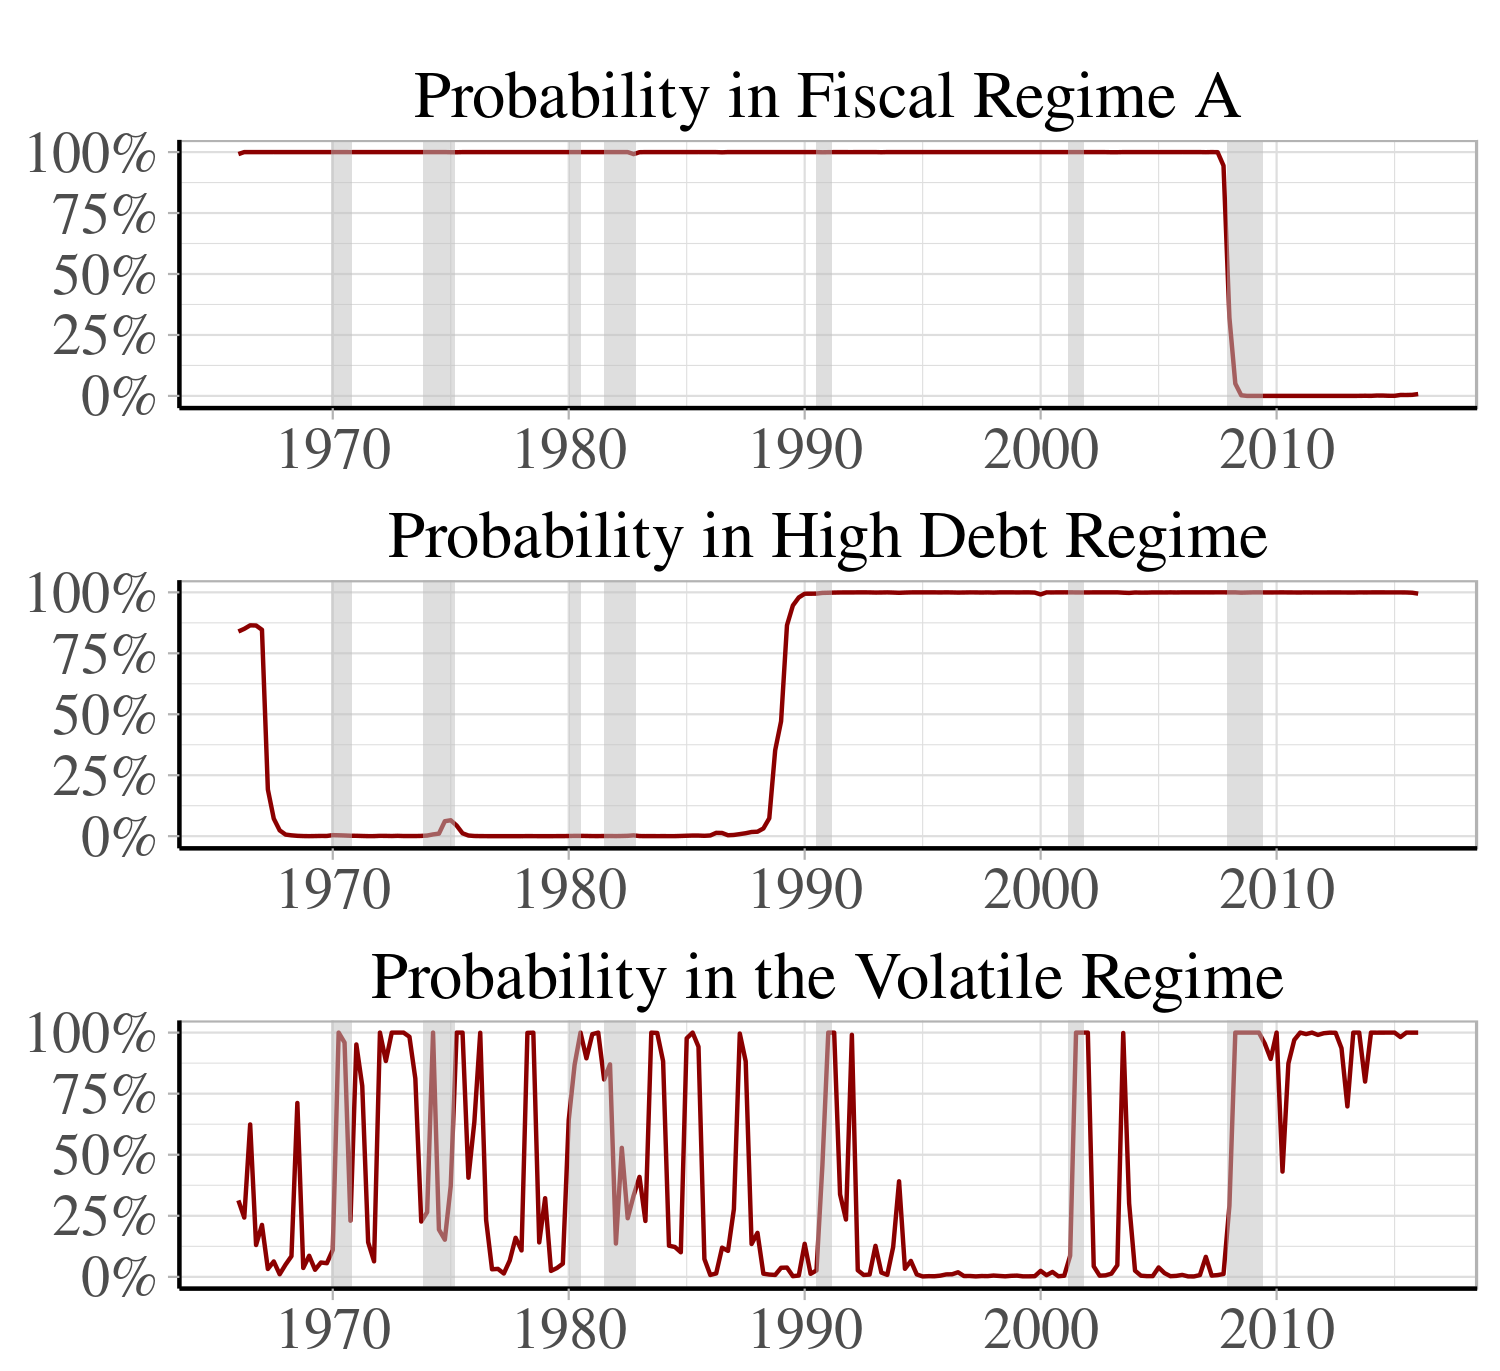
\includegraphics[align=t,height=0.85\textheight]{./plots/regimes.png}\end{center}
\end{frame}

\begin{frame}
  \ft{Examine Impulse Response Functions}
  \small{
  \uncover<+->{\begin{block}{Questions: Compare Differences in Regimes}
      \bi
      \item<+-> Do fiscal policy shocks have different effects on macroeconomic variables in different regimes?
      \item<+-> Do fiscal variables have different interdependent effects in different regimes?
      \item<+-> Do effects of fiscal policy shocks depend on long-run debt target?
      \item<+-> Can we visualize difference of shocks in stable vs. volatile fiscal regimes.
      \ei
        
  \end{block}}

  \uncover<+->{\begin{block}{Left for Future Work}
    \bi
    \item<+-> Long-run effects of moving to a high-debt regime  
    \item<+-> Long-run effects of a change in behavior regime in macroeconomic variables.
    \item<+-> Expectations, behavior, equilibrium effects given regime-switching possibilities.
    \ei
  \end{block}}
  }
\end{frame}


\begin{frame}
  \ft{Fiscal Regimes: Gov Exp Shock}
  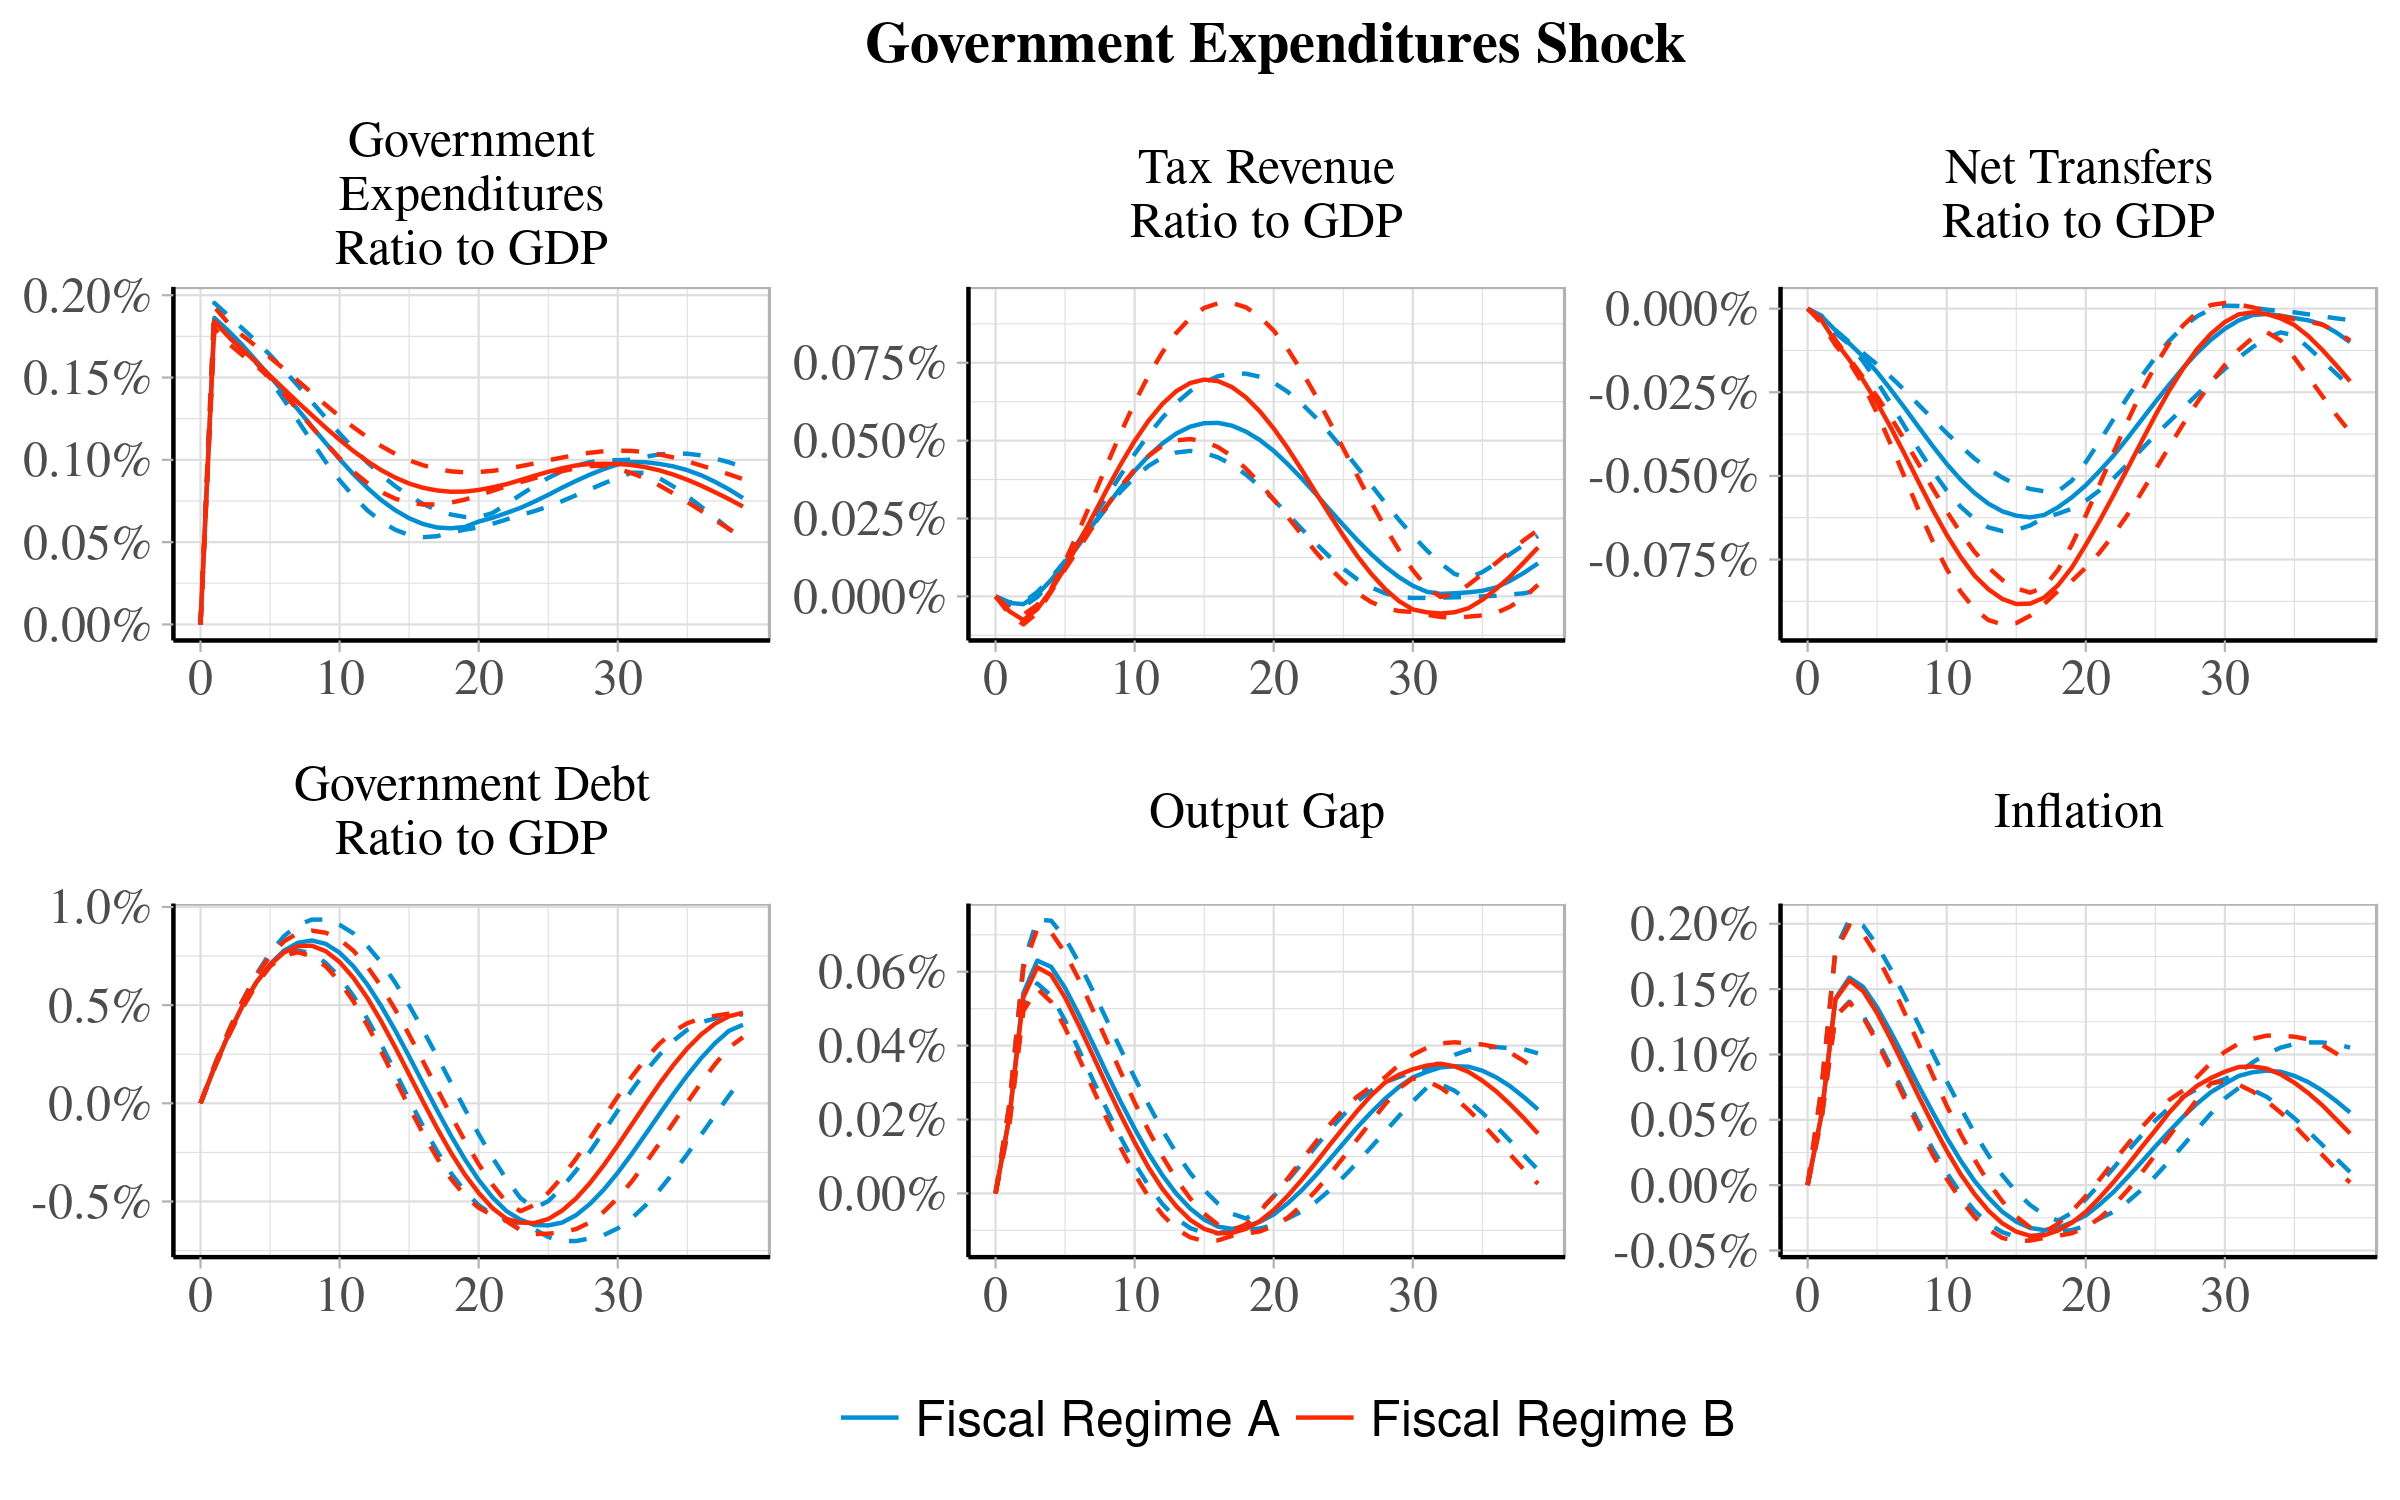
\includegraphics[align=t,width=1.0\textwidth]{./plots/fiscalreg/govirf.png}
  \begin{center}\textcolor{BrickRed}{Smaller response to \textbf{Transfers} in Fiscal Regime A}\\
  \textcolor{BrickRed}{No differences in macroeconomic dynamics}\end{center}
\end{frame}

\begin{frame}
  \ft{Fiscal Regimes: Tax Shock}
  \vspace*{-0.15in}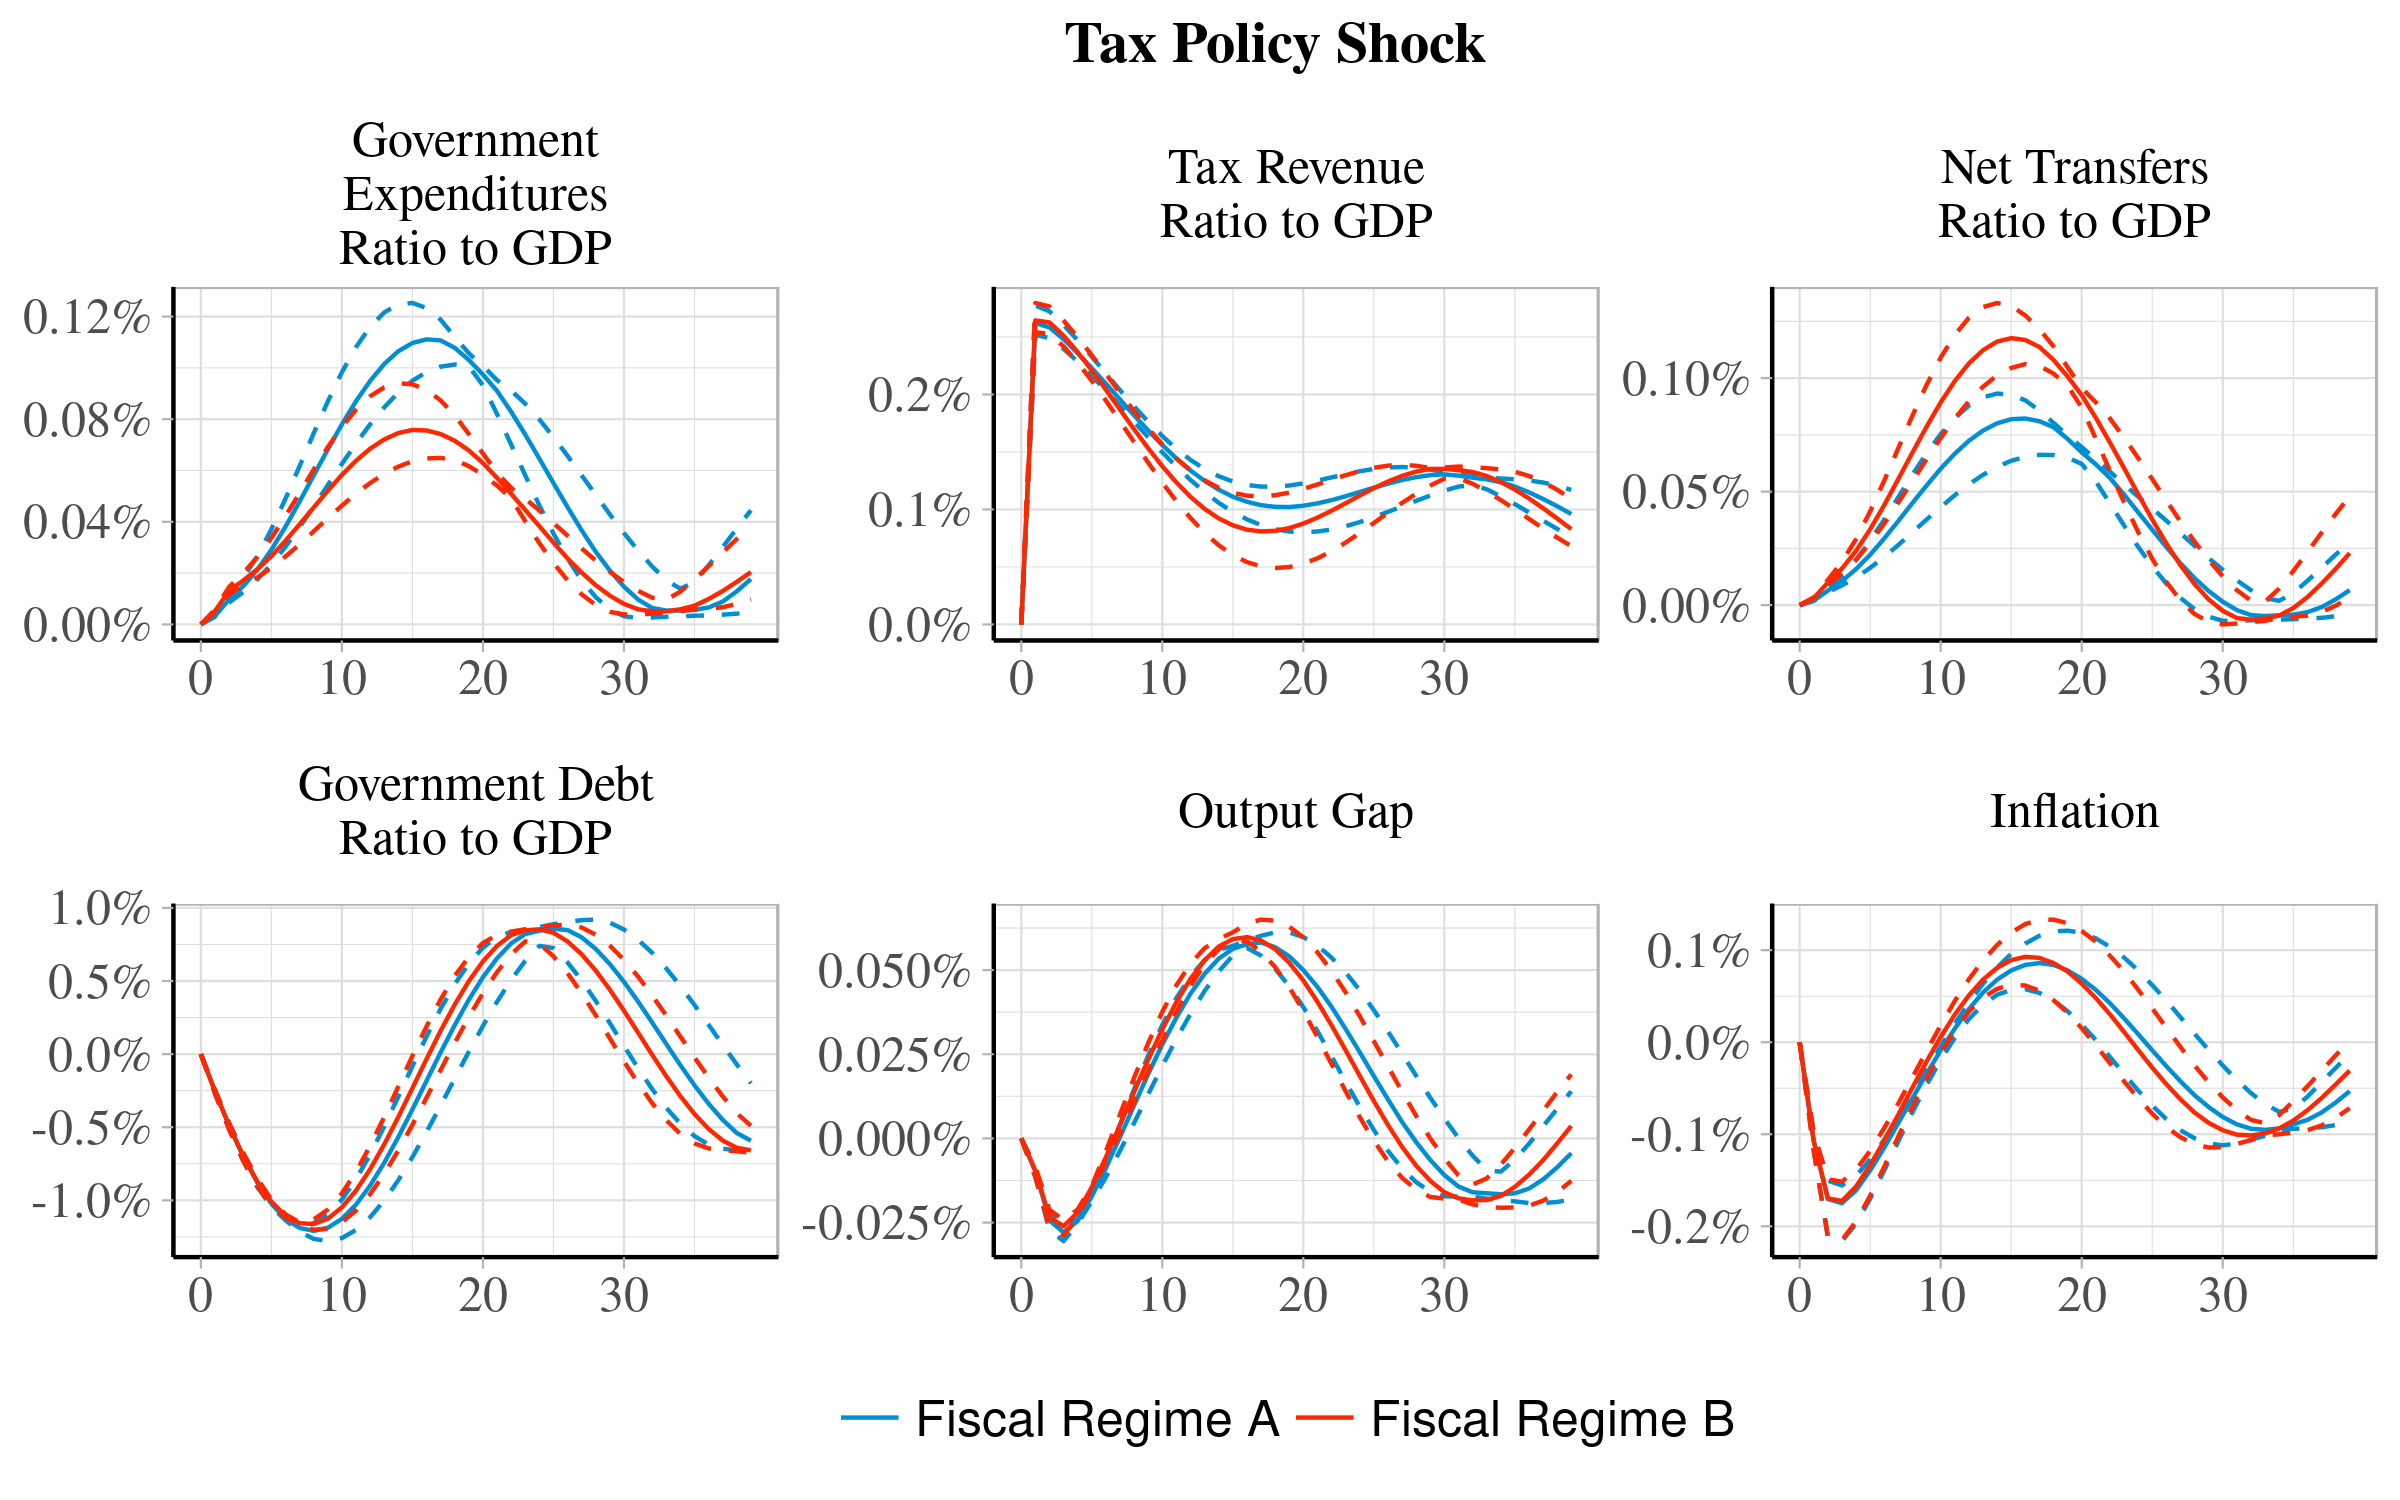
\includegraphics[align=t,width=1.0\textwidth]{./plots/fiscalreg/taxirf.png}
  \begin{center}\textcolor{BrickRed}{Smaller response to \textbf{Transfers} in Fiscal Regime A}\\
    \textcolor{BrickRed}{Larger response to \textbf{Government Expenditures} in Fiscal Regime A}\\
  \textcolor{BrickRed}{No differences in macroeconomic dynamics}\end{center}
\end{frame}

\begin{frame}
  \ft{Fiscal Regimes: Output Gap Shock}
  \vspace*{-0.15in}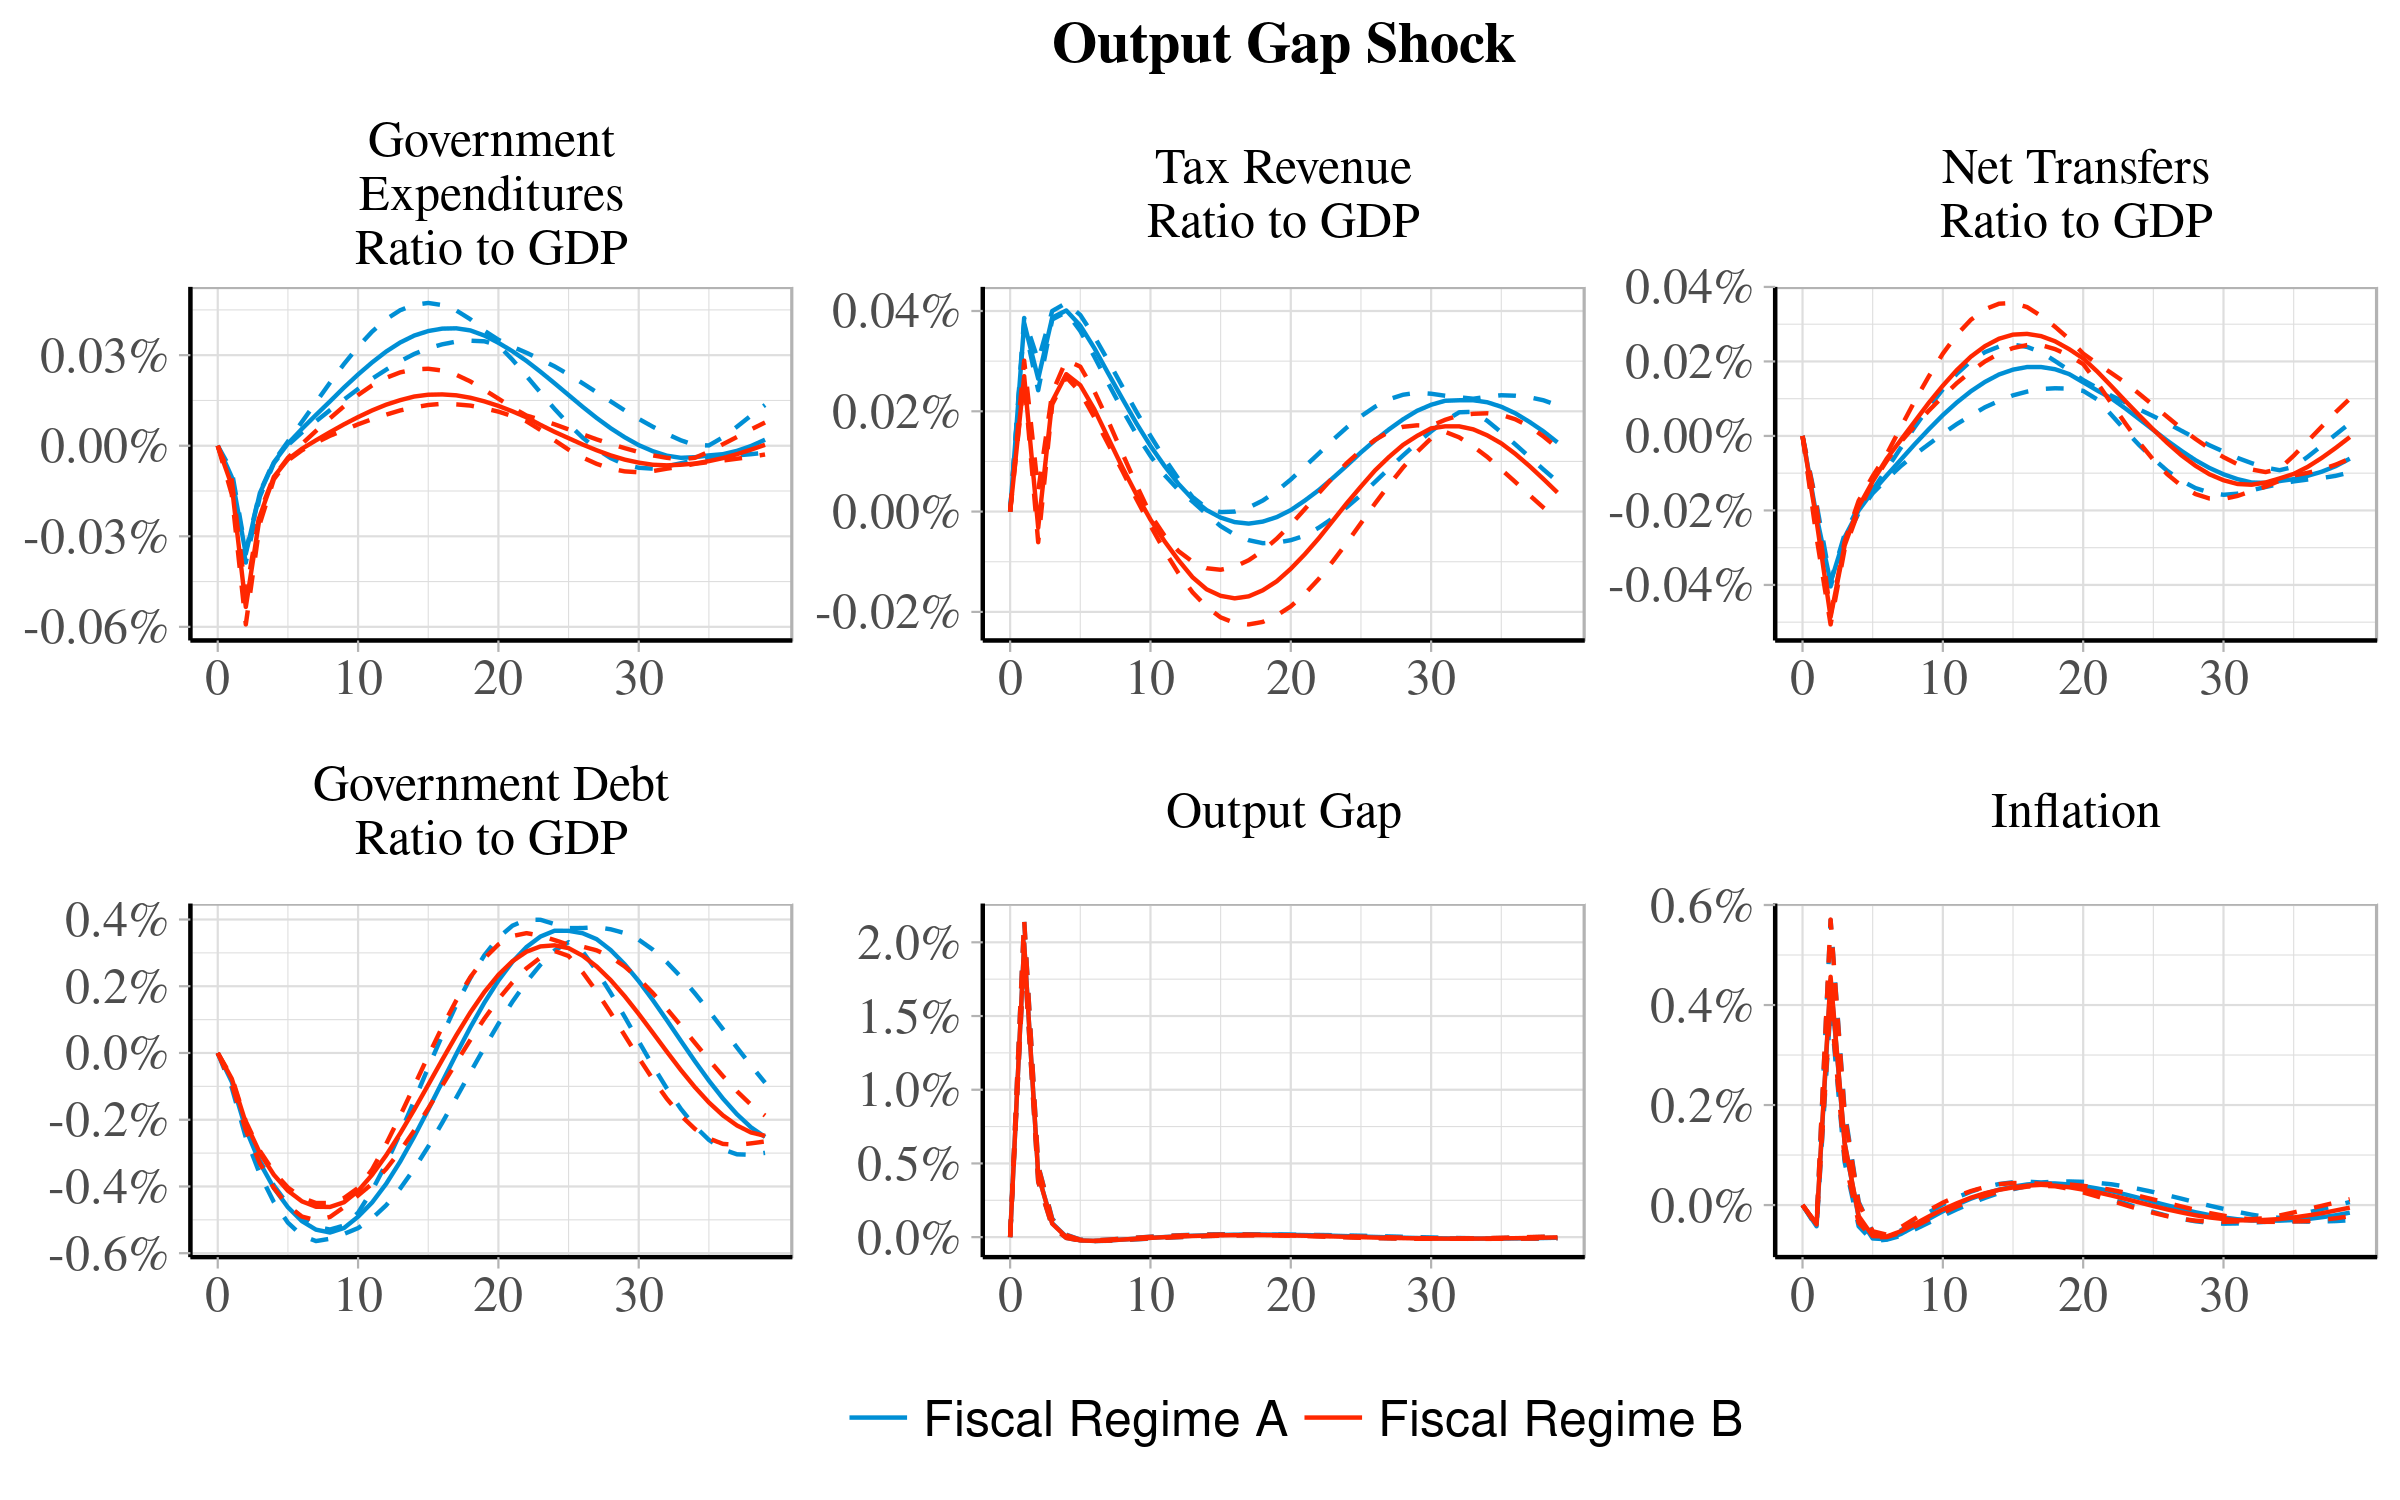
\includegraphics[align=t,width=1.0\textwidth]{./plots/fiscalreg/xirf.png}
  \begin{center}
    \textcolor{BrickRed}{Larger responses to \textbf{Gov Exp} and \textbf{Taxes} in Fiscal Regime A}\\
    \textcolor{BrickRed}{Smaller response to \textbf{Transfers} in Fiscal Regime A}\\
  \textcolor{BrickRed}{No differences in macroeconomic dynamics}
  \end{center}
\end{frame}

\begin{frame}
  \ft{Low/High Debt Regime: Gov Exp Shock}
  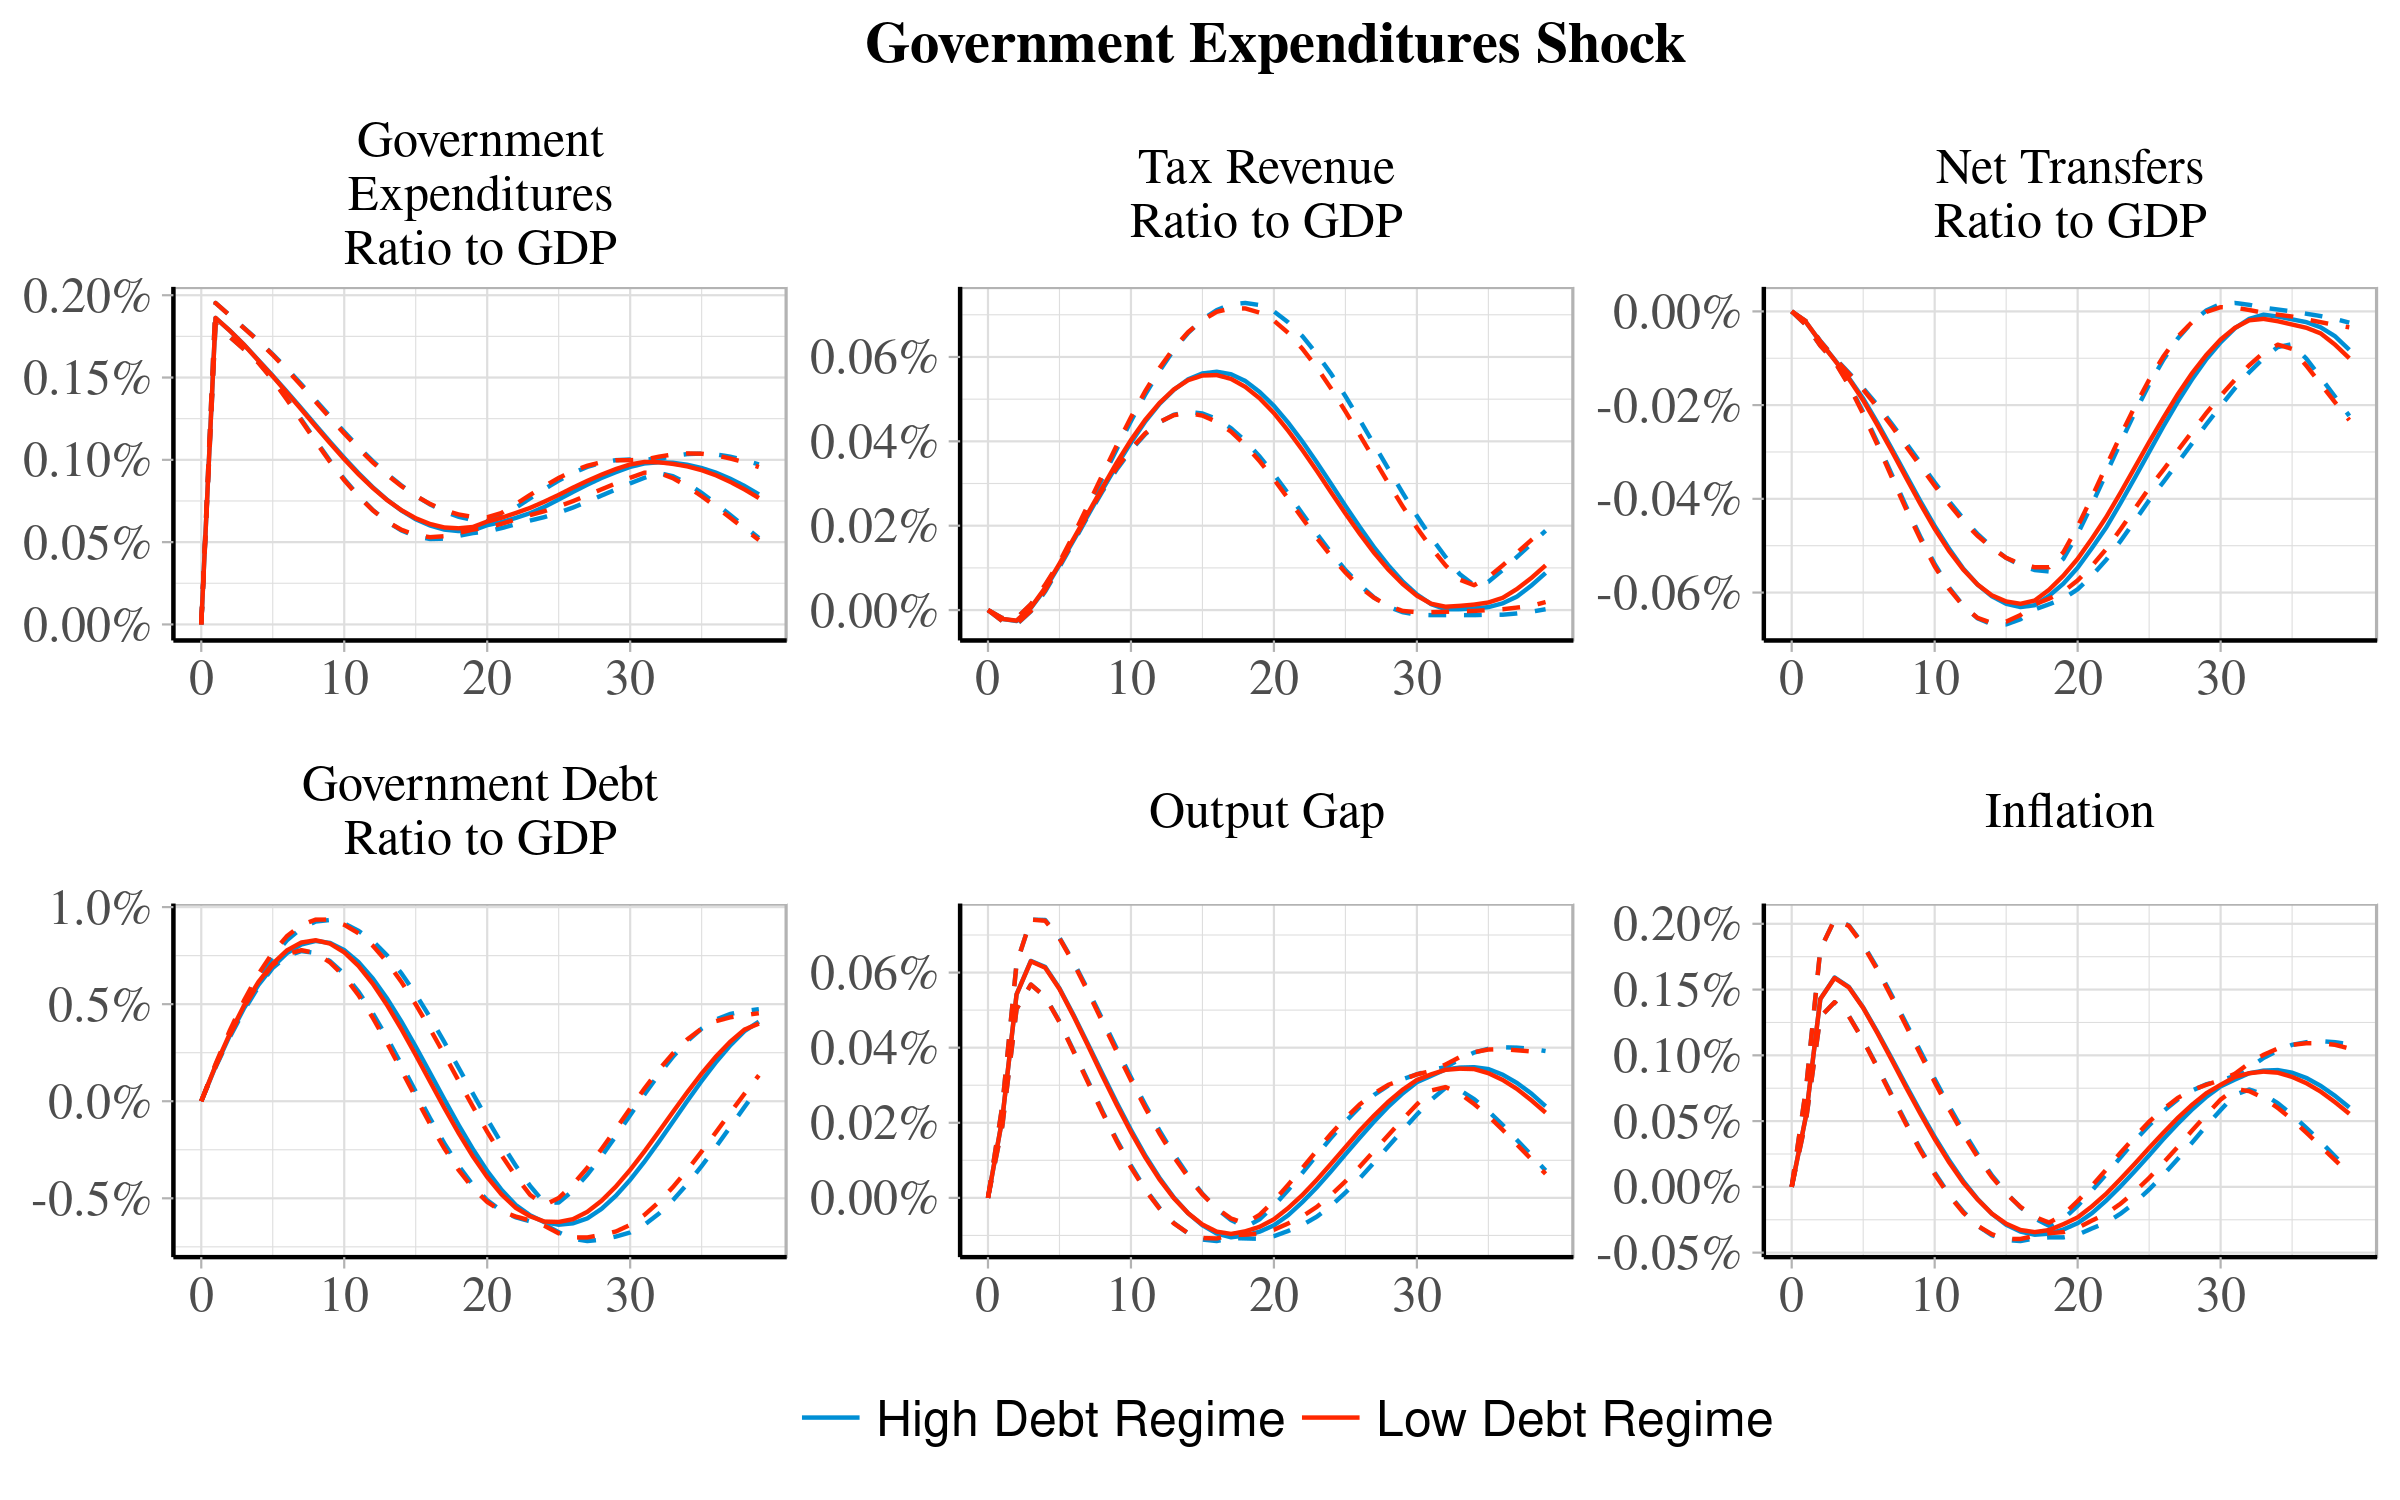
\includegraphics[align=t,width=1.0\textwidth]{./plots/debtreg/govirf.png}
  \begin{center}\textcolor{BrickRed}{Debt regime affects neither fiscal or macroeconomic dynamics}\end{center}
\end{frame}

\begin{frame}
  \ft{Low/High Debt Regime: Tax Shock}
  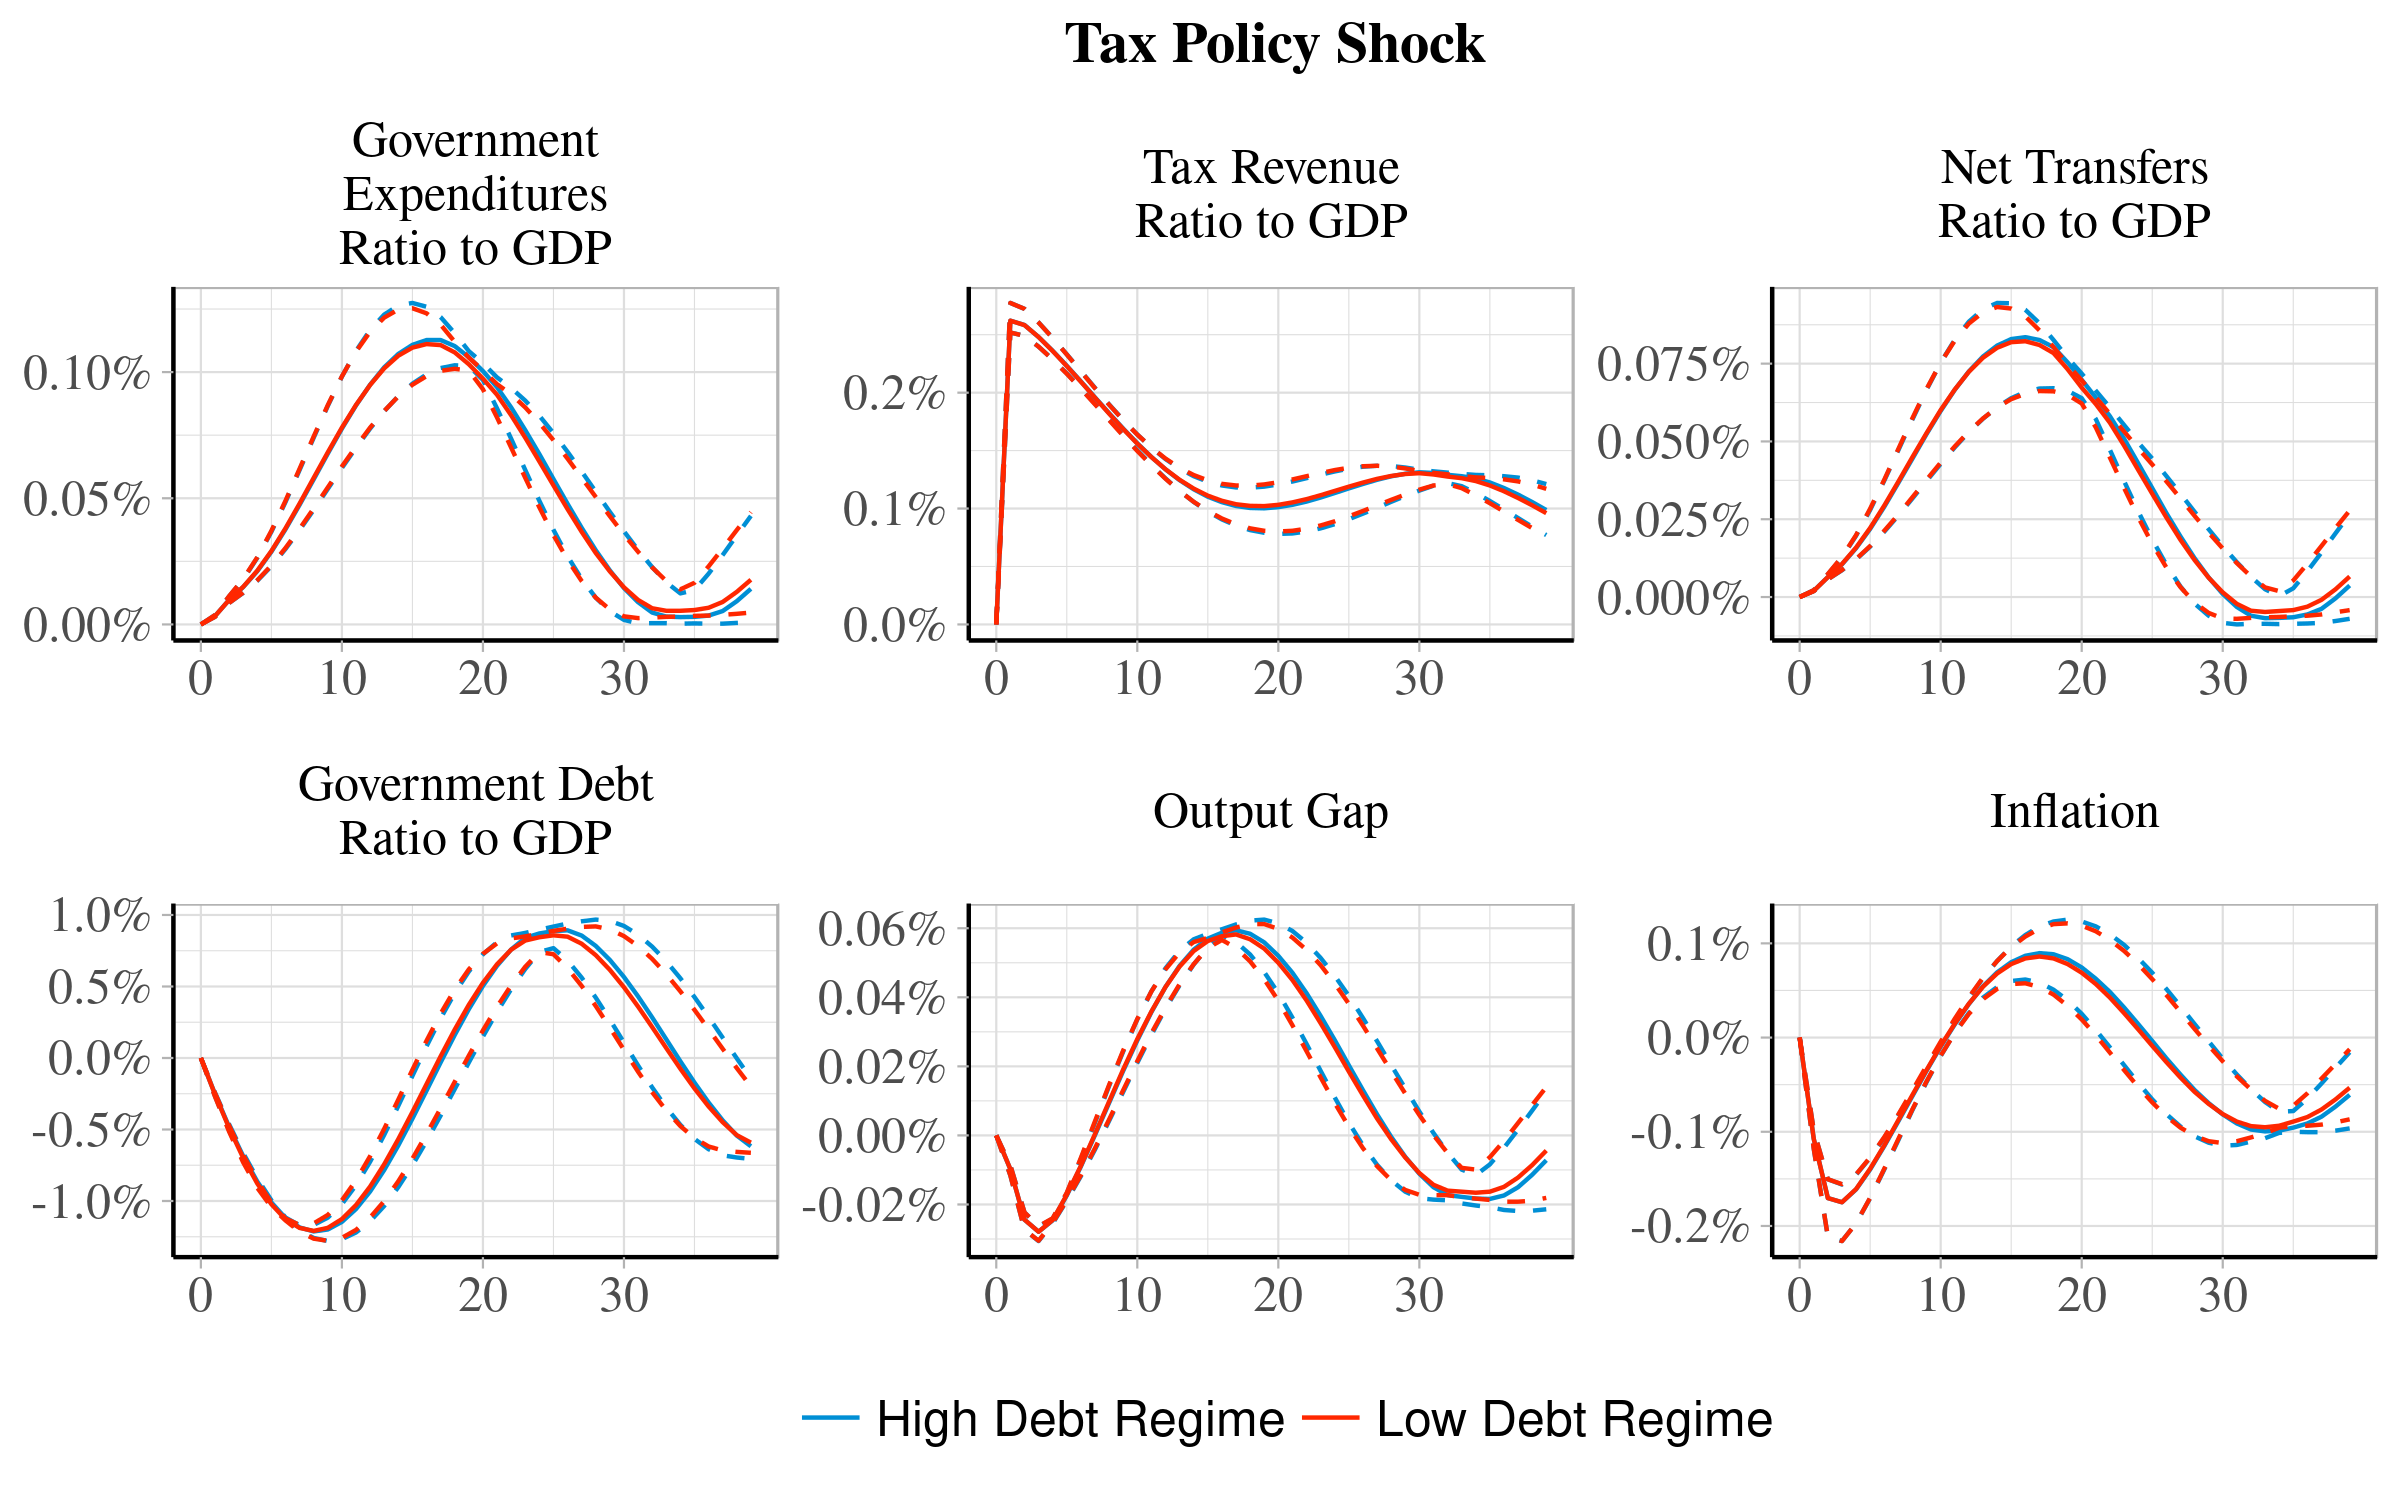
\includegraphics[align=t,width=1.0\textwidth]{./plots/debtreg/taxirf.png}
  \begin{center}\textcolor{BrickRed}{Debt regime affects neither fiscal or macroeconomic dynamics}\end{center}
\end{frame}

\begin{frame}
  \ft{Low/High Debt Regime: Output Gap Shock}
  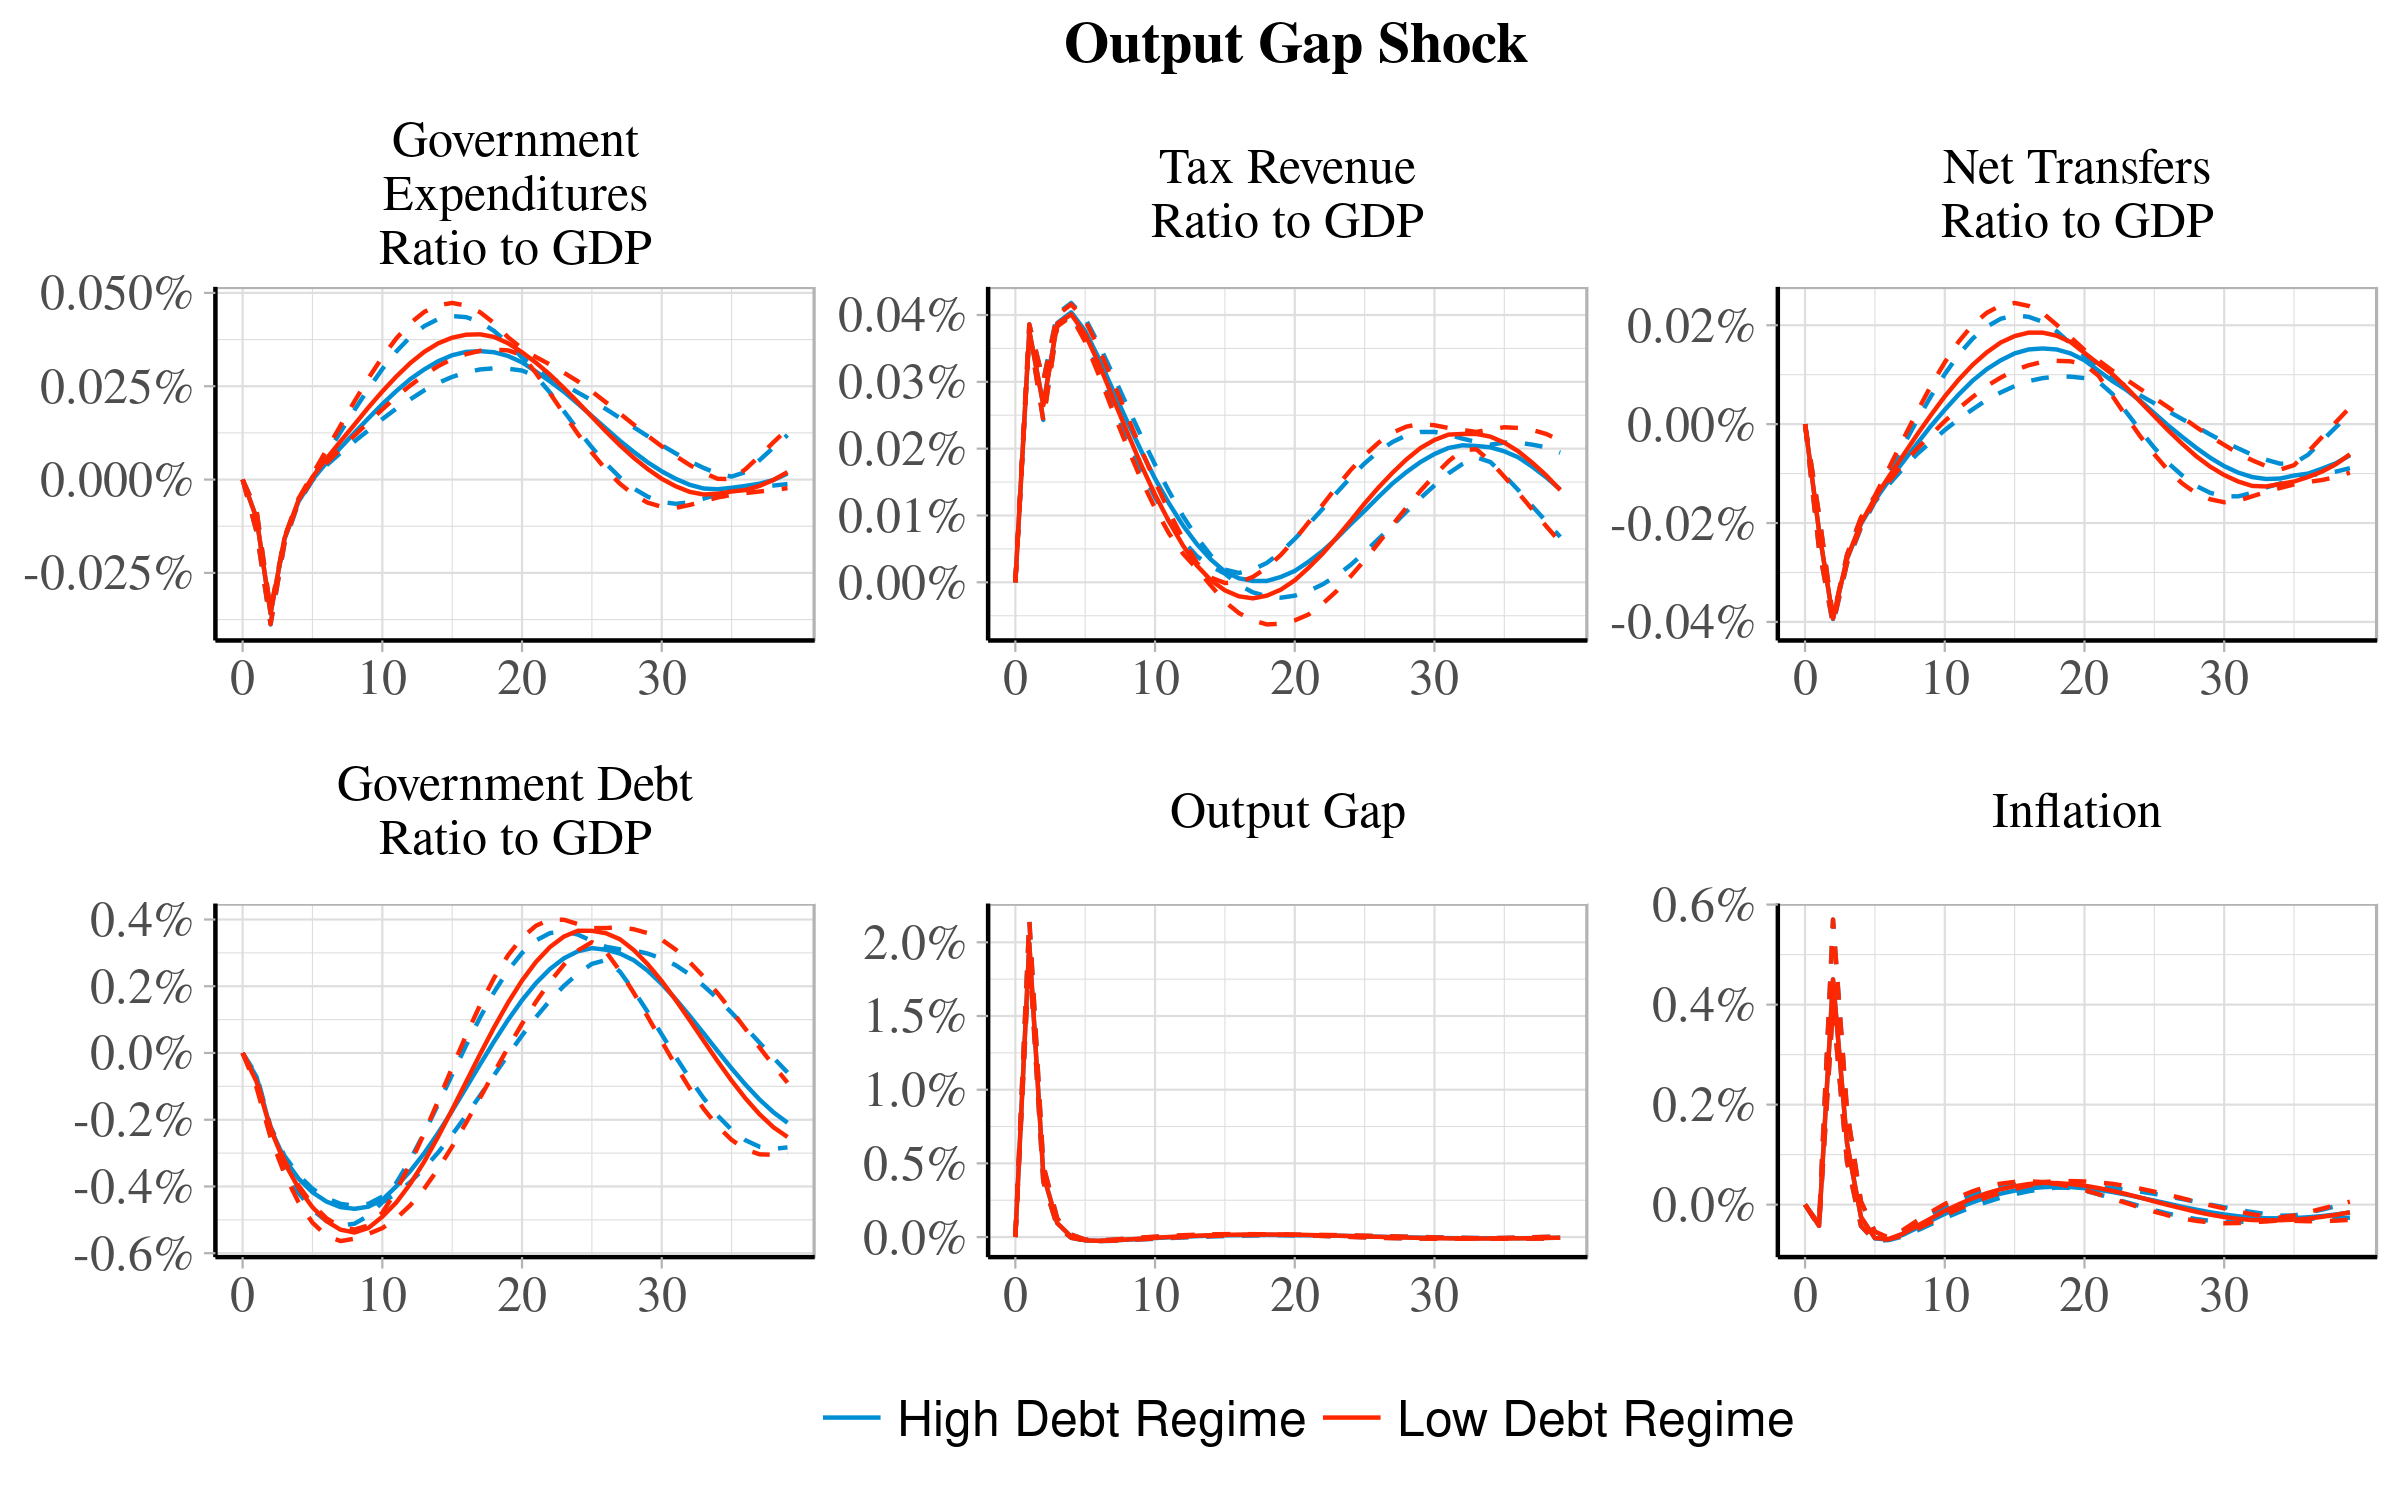
\includegraphics[align=t,width=1.0\textwidth]{./plots/debtreg/xirf.png}
  \begin{center}\textcolor{BrickRed}{Debt regime affects neither fiscal or macroeconomic dynamics}\end{center}
\end{frame}

\begin{frame}
  \ft{Fiscal Volatility Regimes: Gov Exp Shock}
  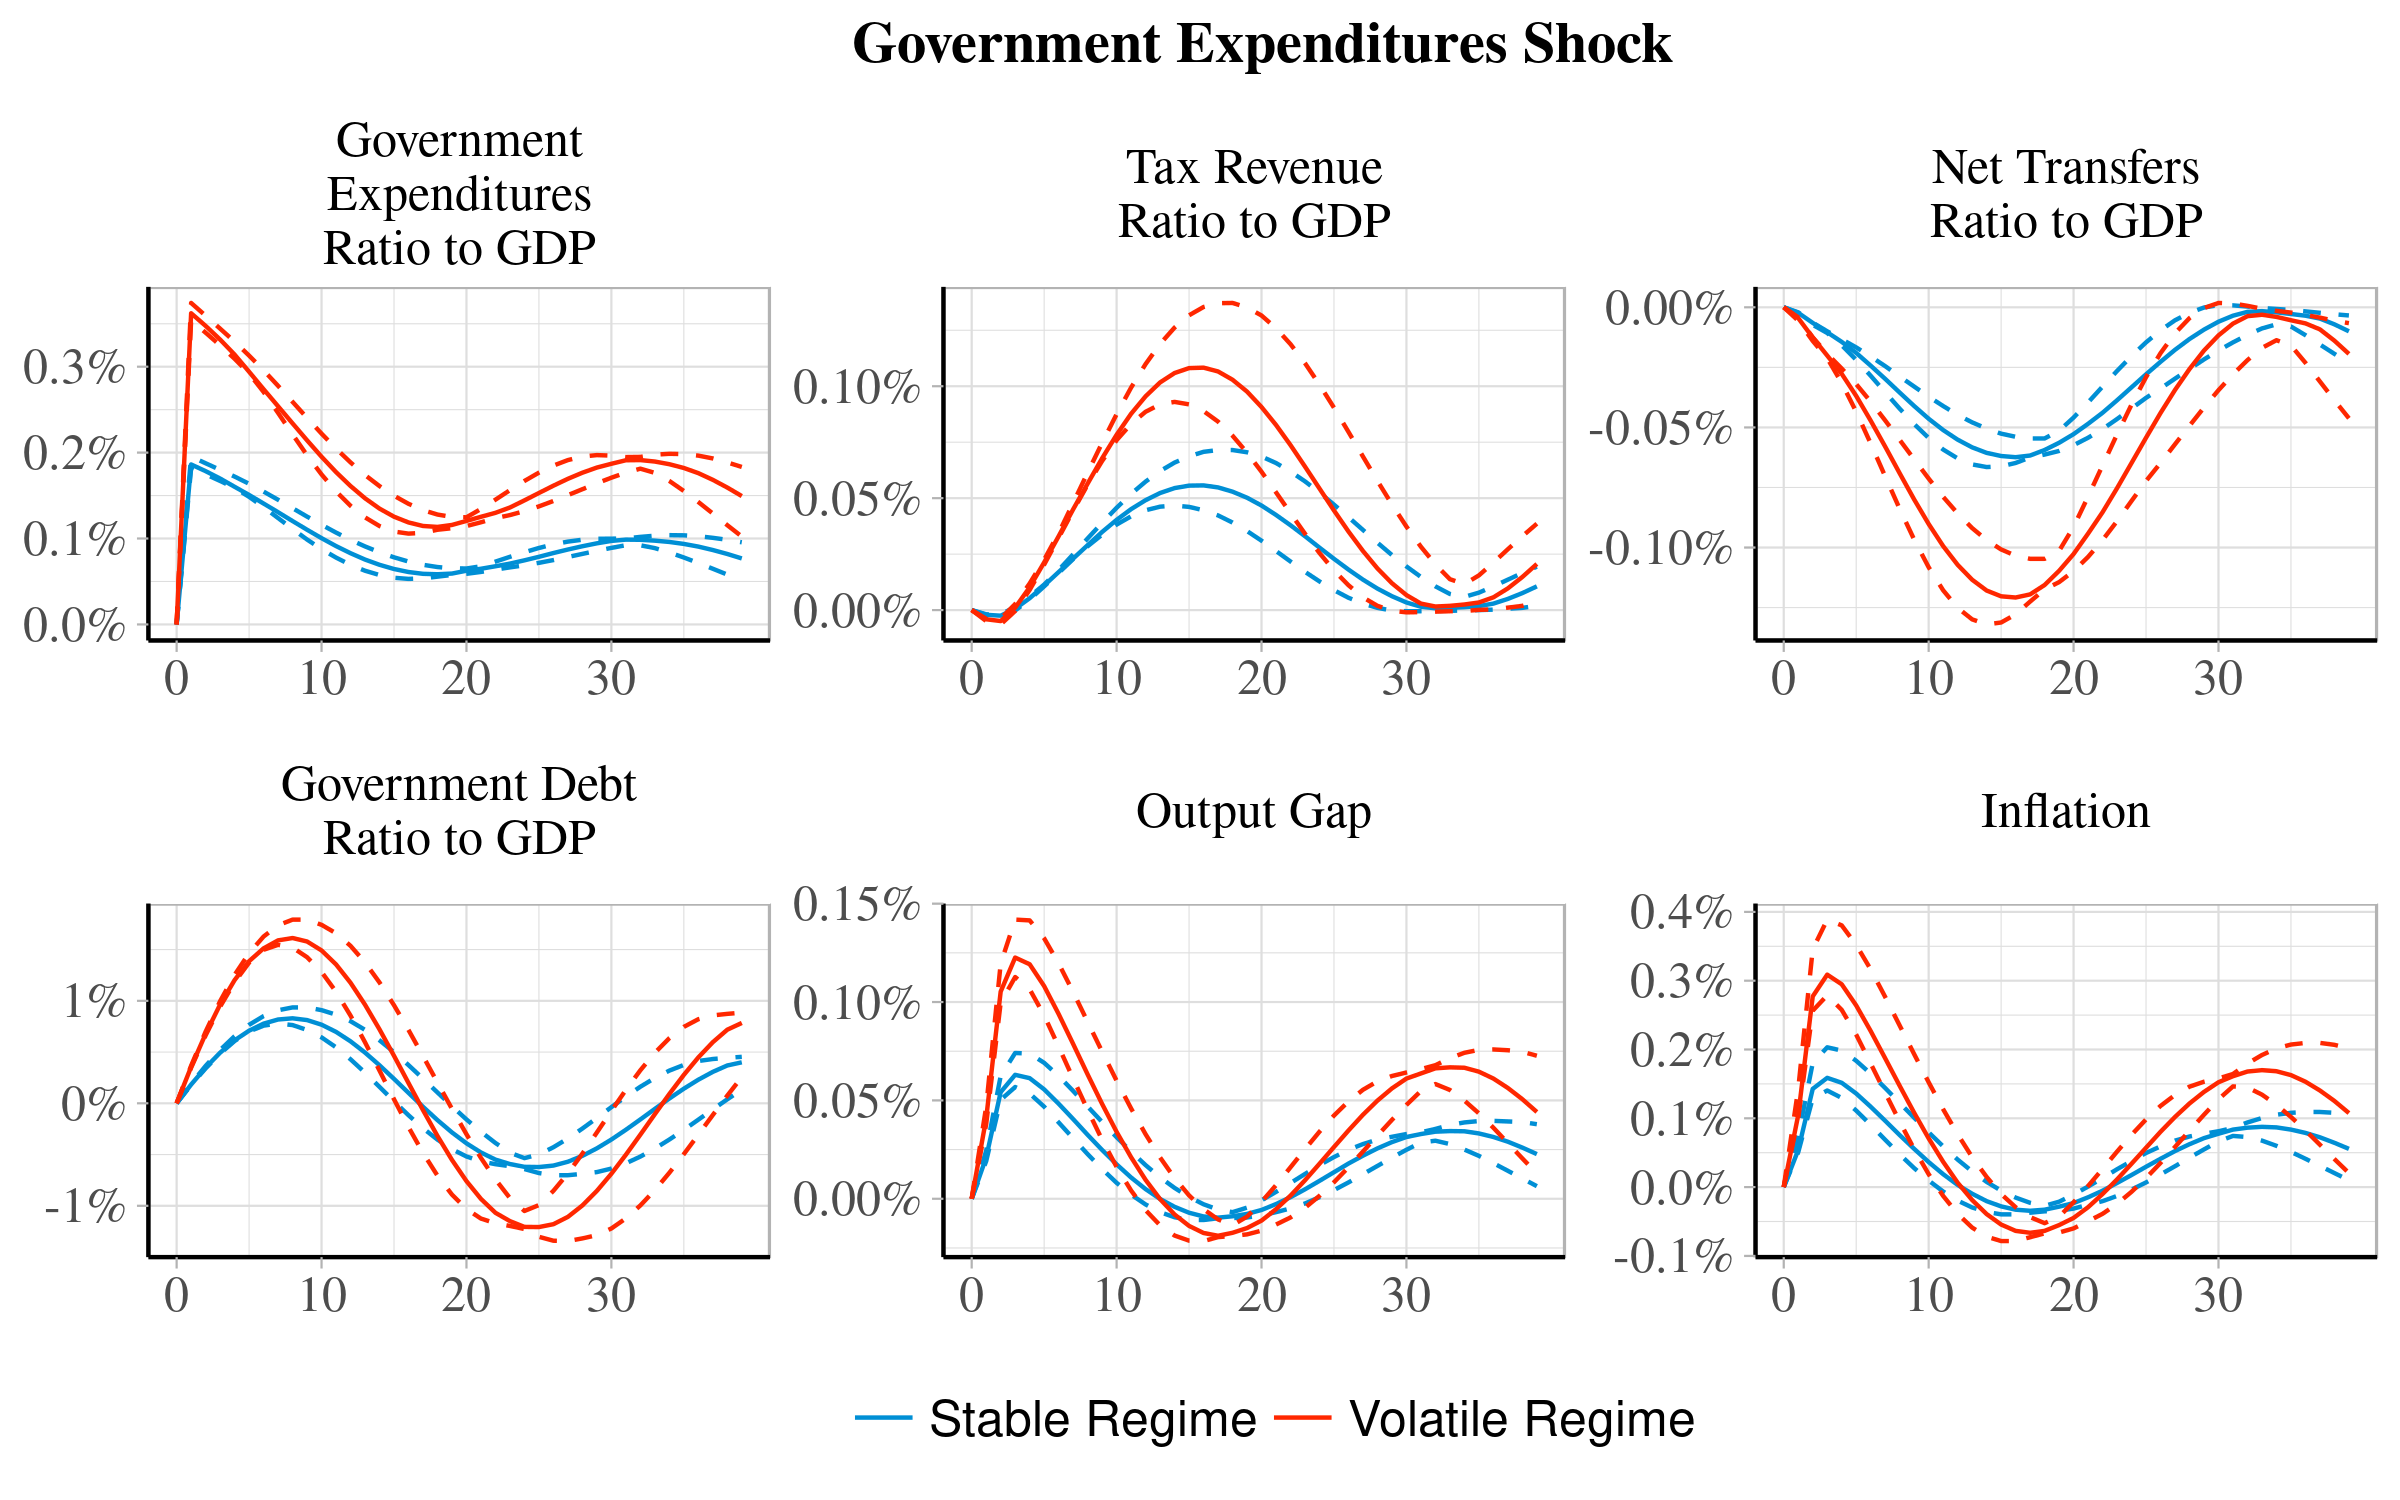
\includegraphics[align=t,width=1.0\textwidth]{./plots/volreg/govirf.png}
  \begin{center}\textcolor{BrickRed}{Much larger sized shocks and responses in volatile regime}\end{center}
\end{frame}

\begin{frame}
  \ft{Fiscal Volatility Regimes: Tax Shock}
  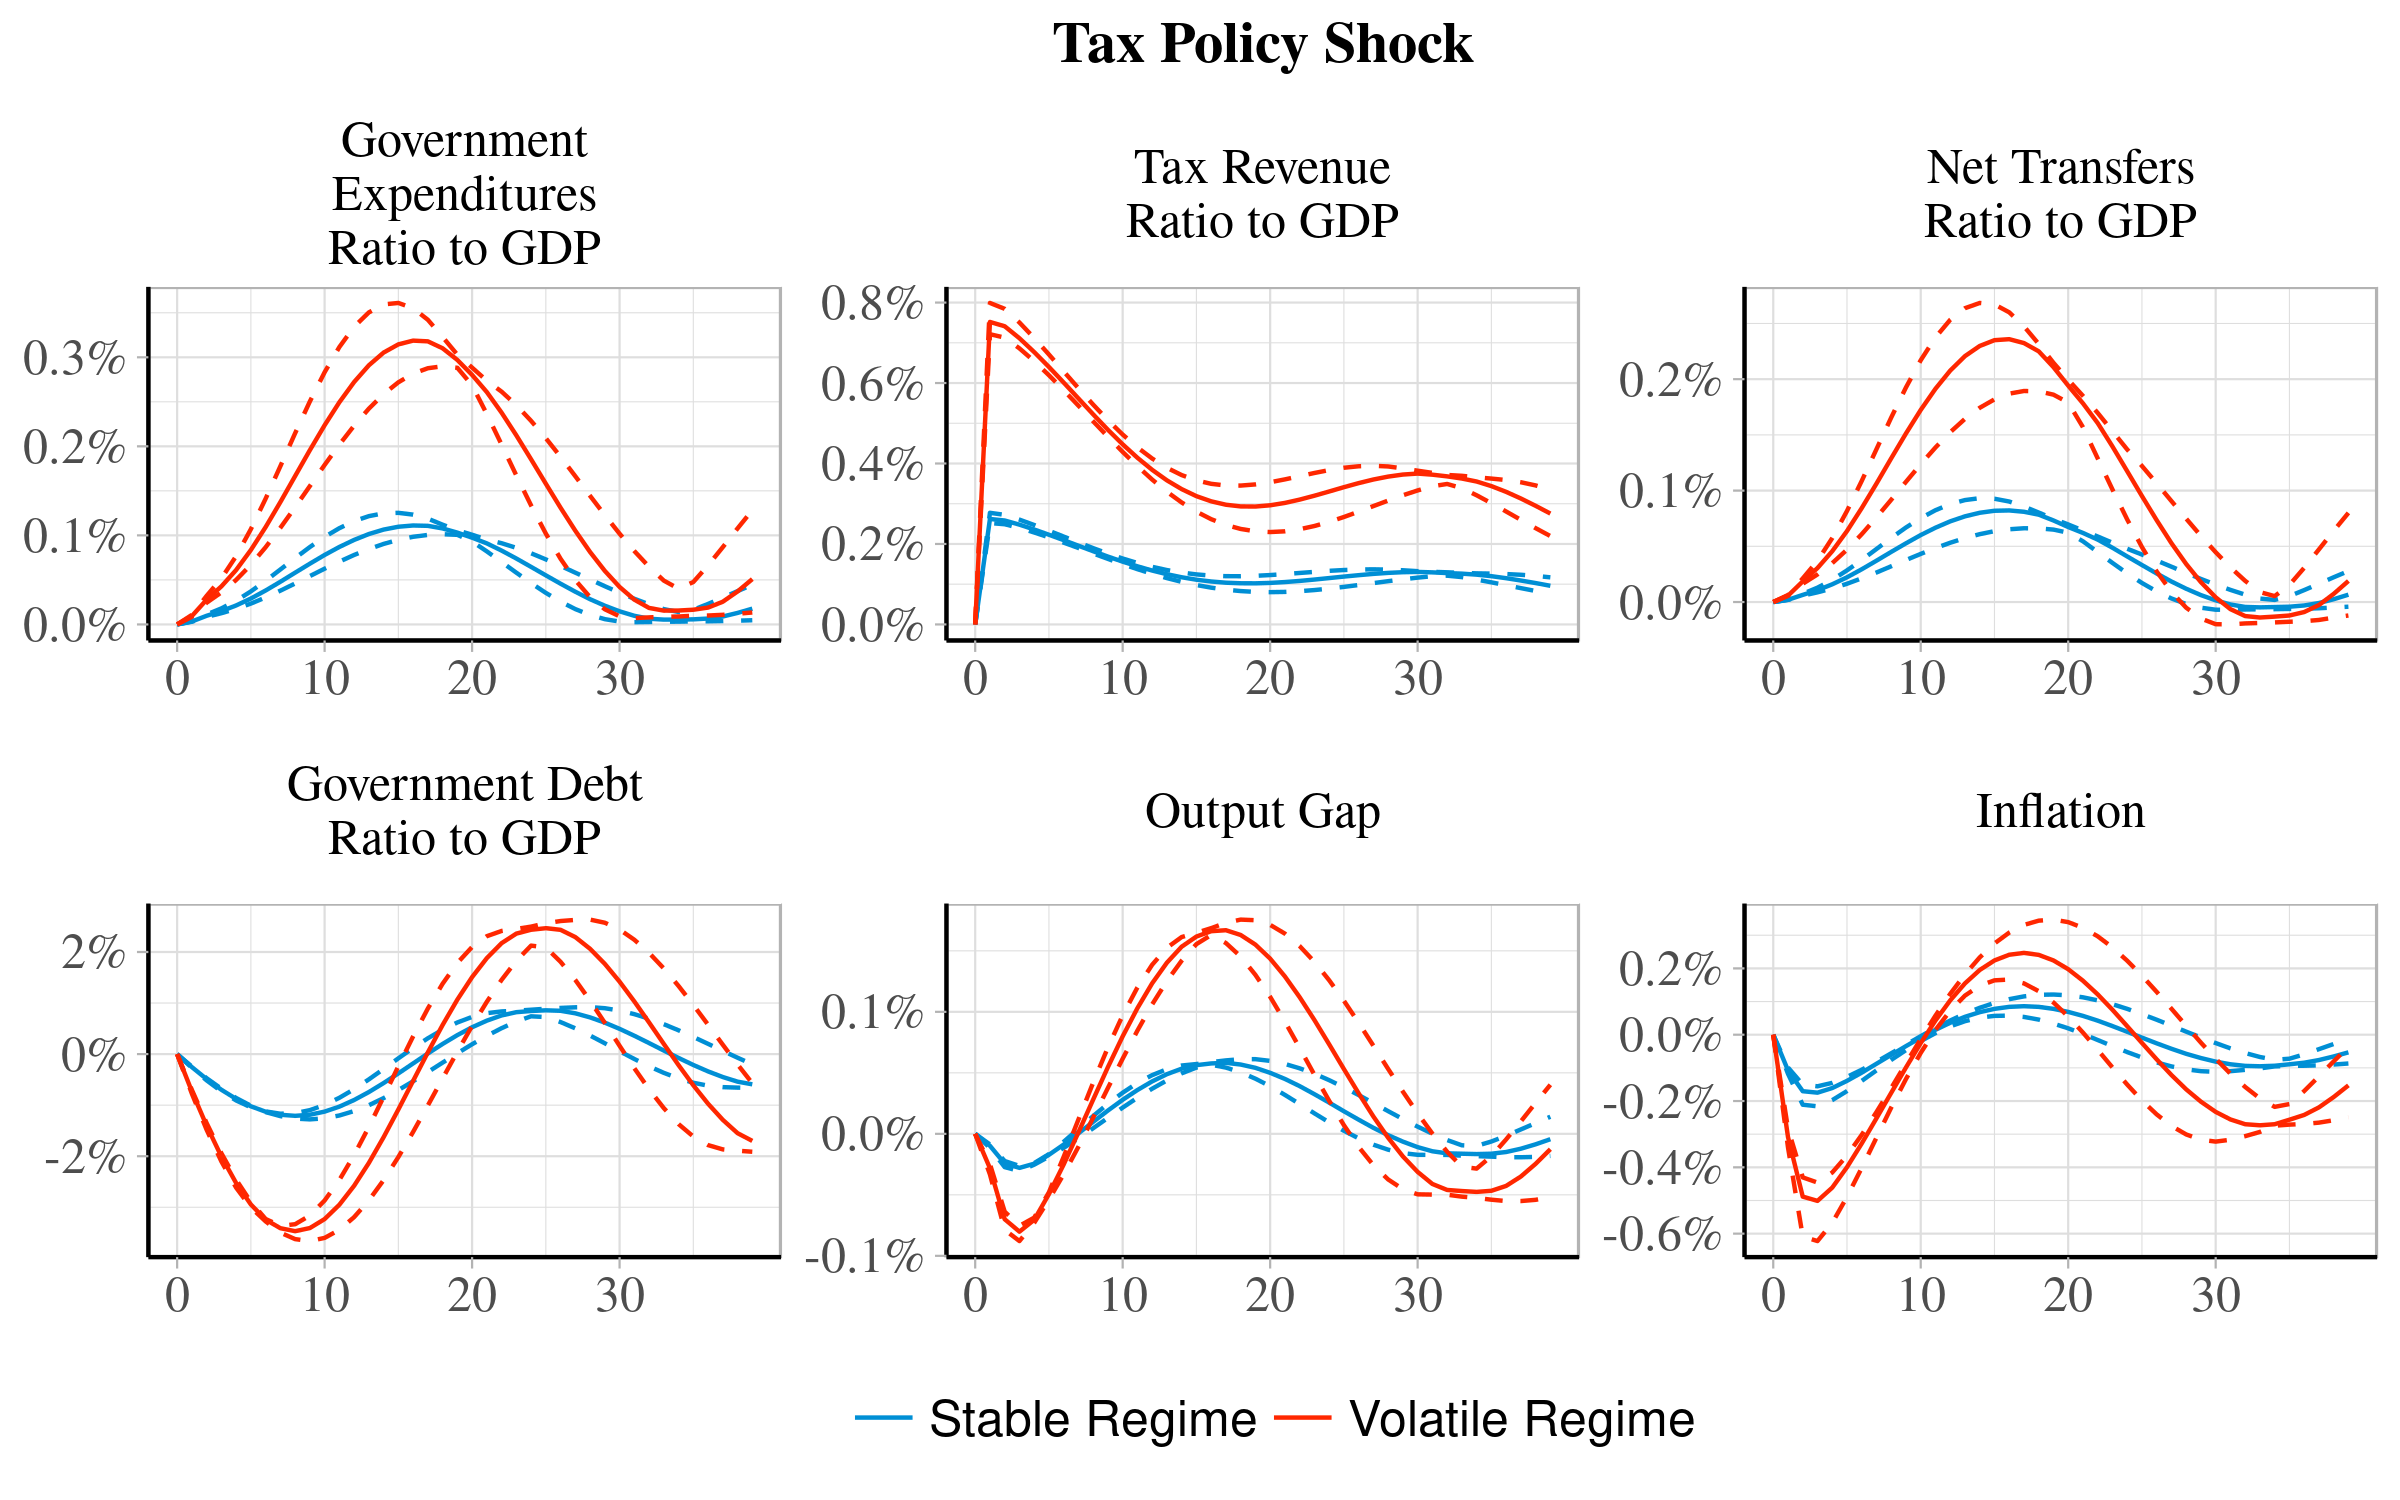
\includegraphics[align=t,width=1.0\textwidth]{./plots/volreg/taxirf.png}
  \begin{center}\textcolor{BrickRed}{Much larger sized shocks and responses in volatile regime}\end{center}
\end{frame}

\begin{frame}
  \ft{Fiscal Volatility Regimes: Transfer Shock}
  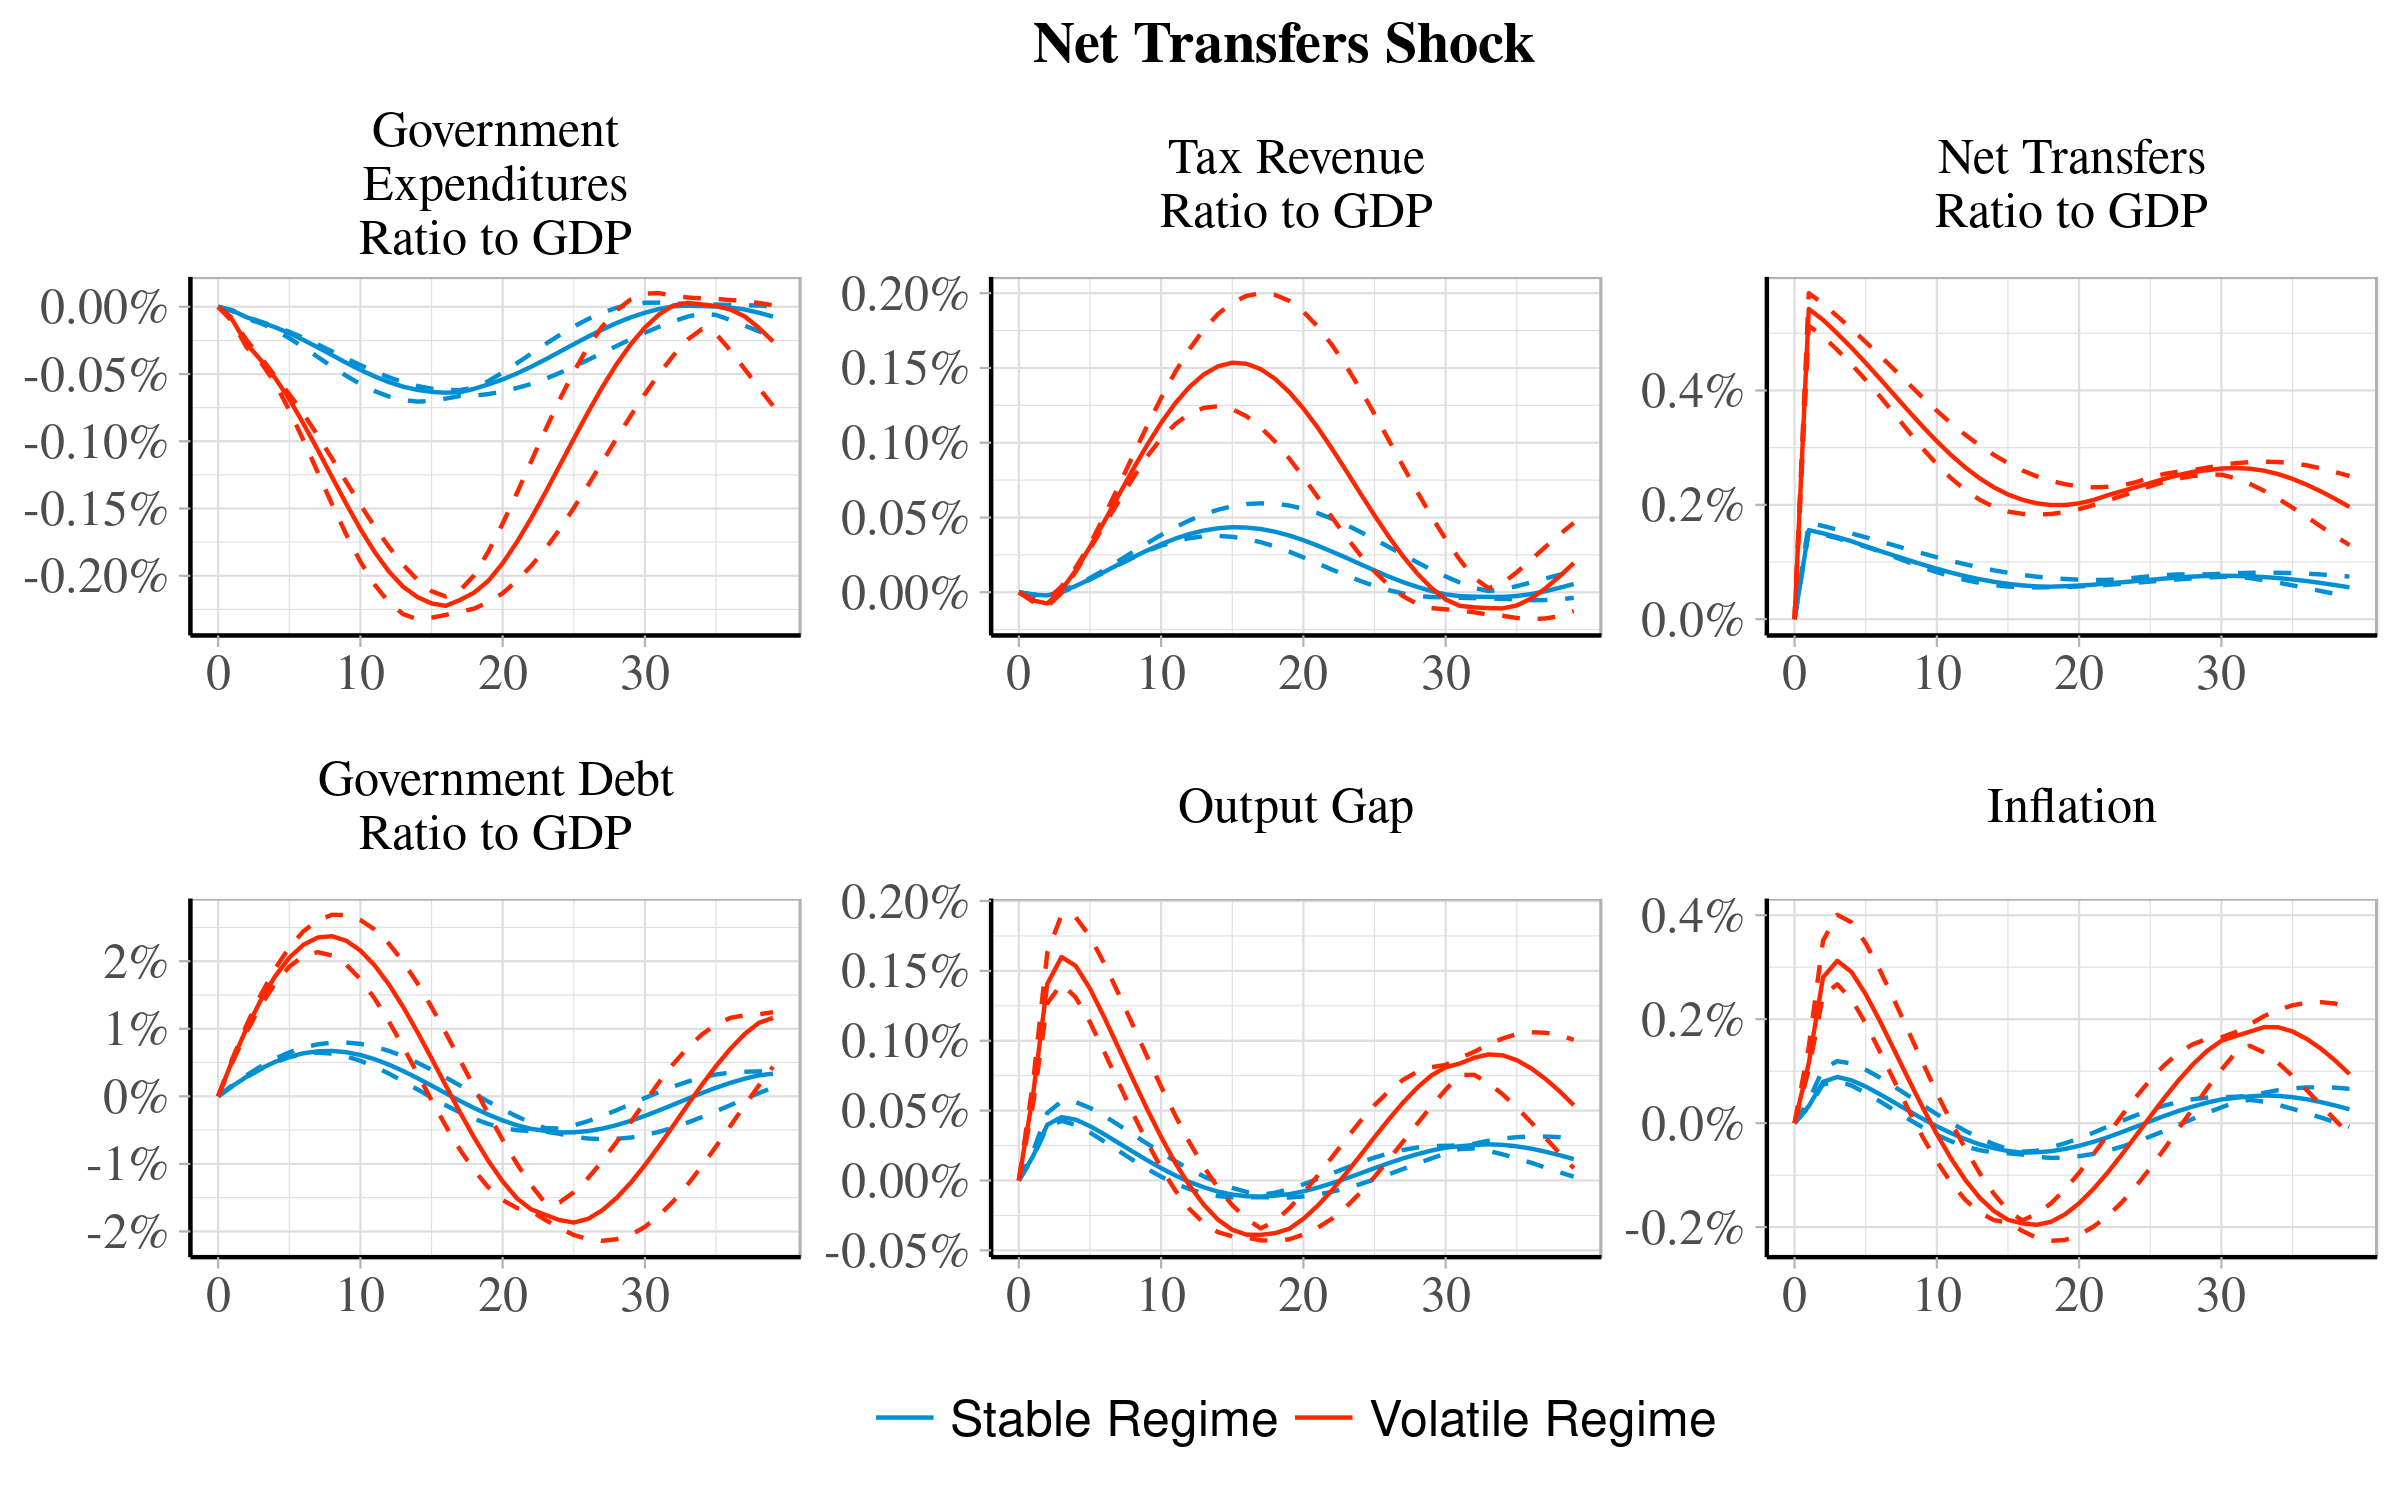
\includegraphics[align=t,width=1.0\textwidth]{./plots/volreg/transferirf.png}
  \begin{center}\textcolor{BrickRed}{Much larger sized shocks and responses in volatile regime}\end{center}
\end{frame}

\begin{frame}
  \ft{Conclusions}
  \bi
  \item<+-> Evidence of switching in all three dimensions.
  \item<+-> Switch from low-debt to high-debt regime in 1989.
  \item<+-> Single, permanent, switch in fiscal policy behavior in 2008.
    \bi
    \item Government expenditures playing larger role in macroeconomic stabilization, smaller role in balancing budget.
    \item Taxes play smaller role in macroeconomic stabilization, larger role in balancing budget.
      \ei
  \item<+-> Many switches from stable to volatile fiscal regimes, usually around and following recessions.
  \item<+-> Differences in impulse response functions explained mostly by changing fiscal volatility.
  \ei   
\end{frame}


\end{document}

